\documentclass{bioinfo}
\usepackage{hyperref}
\usepackage{pifont}
\usepackage{amsfonts}
\usepackage{subfigure}
\usepackage{multirow}
\usepackage{booktabs}
\usepackage{array}
\usepackage{float}
\usepackage{graphicx}
\usepackage{epstopdf}
\usepackage{color}
\usepackage{tabularx,caption}
\usepackage{amsmath}
\usepackage{bm}
\usepackage{mathtools}
\usepackage{threeparttable}
\usepackage{stfloats}
\usepackage{bbm}
\usepackage[marginal]{footmisc}
% \renewcommand{\thefootnote}{}

% \copyrightyear{2017} \pubyear{2017}
% \access{Advance Access Publication Date: Day Month Year}
% \appnotes{Manuscript Category}

\begin{document}

\begin{methods}
\section{Abstract}
Circular non-coding RNA (circRNA) is closely associated with various human diseases. Identifying disease-related circRNAs can provide deeper insights into the pathogenesis of diseases. Advanced prediction methods for circRNA-disease associations mainly focus on graph learning techniques such as graph convolutional networks and graph attention mechanisms. However, these methods do not fully encode the multi-scale neighbor topology among nodes. We propose a \textbf{m}ulti-scale neighbor topology-guided transformer and \textbf{K}AN enhanced feature learning-based \textbf{c}ircRNA and \textbf{d}isease association prediction model (MKCD) to integrate multi-scale neighbor topology, complex relationships among multiple nodes, and the global and local dependencies of node pair attributes.
First, MKCD incorporates an adaptive random walk with restart (ARWR) component, which can construct neighbor topologies covering different scopes of neighbors by random walking on the circRNA-disease-miRNA heterogeneous graph. 
Second, we introduce a dynamic multi-scale neighbor topology-guided transformer (DMTT), which leverages the multi-scale neighbor topology to guide the learning of relationships among circRNA, miRNA, and disease nodes. The multi-scale neighbor topology is dynamically evolving, guiding the transformer's learning process in a dynamic manner.
Third, we establish a feature gated network (FGN) to understand the importance of the topological features derived from DMTT and the original features of the nodes.
Finally, we propose an adaptive Kolmogorov-Arnold network and convolutional neural networks combination learning strategy to learn the global and local dependencies of features between circRNA and disease node pairs. 
The comprehensive comparison experiments demonstrated our method's superior prediction performance compared to six advanced methods, and ablation experiments showed the effectiveness of ARWR, DMTT, FGN, and ACK. Case studies over three diseases further confirmed the application value of our method in discovering reliable circRNA candidates for the diseases of interest.

%---------------------------------------------------------------------------------------------------------------------


\section{Introduction}
\textcolor{blue}{CircRNA is a class of single-stranded circular non-coding RNA without 5' and 3' polyadenylated tails \cite{jeck2014detecting}. Increasing evidence suggests that the abnormal expression of circRNAs is associated with the occurrence of various diseases \cite{abdelmohsen2017identification}, including cancers \cite{gao2019circular, li2019tumor, liang2020autophagy}, immune system disorders \cite{wang2018circibtk}, and cardiovascular diseases \cite{khan2016rbm20, siede2017identification, jin2019silencing}. Therefore, identifying the associations between diseases and circRNAs can aid in the diagnosis and treatment of these diseases. Computational prediction methods can help discover associations between circRNAs and diseases and provide reliable disease-related circRNA candidates for subsequent biological experiments \cite{lan2023benchmarking, yang2021predicting}.}

\textcolor{blue}{Existing computational prediction methods can be categorized into three main types. The first type involves establishing network-based models to predict the associations between circRNAs and diseases. The KATZHCDA and PWCDA models calculate the association scores for each circRNA-disease pair based on the paths connecting them in heterogeneous networks \cite{fan2018prediction, lei2018pwcda}. The iCircDA-MF model proposed by Wei et al. incorporates gene information to construct a circRNA-gene-disease relationship network and makes predictions based on matrix factorization \cite{wei2020icircda}. However, these models suffer from limited association information.}

\textcolor{blue}{The second category of prediction models is based on machine learning techniques to infer the associations between circRNAs and diseases. Several methods combine k-nearest neighbors to predict circRNA candidates related to diseases \cite{wang2022combining, lei2020integrating, yan2018dwnn}. The MLCDA model proposed by Wang et al. performs predictions through inductive matrix completion \cite{wang2022machine}. GBDTCDA and AE-RF are both decision tree-based prediction methods \cite{lei2019gbdtcda, deepthi2021inferring}, while CD-LNLP and RNMFLP calculate the association scores between circRNAs and diseases through label propagation \cite{zhang2019predicting, peng2022rnmflp}. However, these methods establish shallow prediction models, making it difficult to learn the deep relationships between circRNAs and diseases.}

\textcolor{blue}{The third category focuses on developing models based on deep learning strategies, further enhancing prediction performance by extracting complex and representative features. Several methods establish convolutional neural network (CNN)-based models to predict disease-related circRNAs \cite{tian2024mamlcda, wang2020efficient, lu2020improving}, yet they overlook the neighbor topology structure among multiple circRNA and disease nodes. The Bi-SGTAR proposed by Li et al. employs an encoder with sparse gating to infer the propensity of all circRNA-disease associations \cite{li2024bi}. This method also neglects the topology formed by circRNA and disease nodes. Other methods are based on graph convolutional networks \cite{shang2024sgfccda, liu2023mpclcda, wu2022mdgf} and graph attention networks \cite{wu2023mlngcf}, as well as combinations of both \cite{dai2022graphcda}, to learn deep features of nodes. However, these methods learn the features of each node from the entire graph, ignoring the global dependency learning of features between individual circRNA and disease node pairs.}

We propose a novel circRNA-disease association prediction model, MKCD, aimed at learning the multi-scale neighbor topology, the relationships among multiple circRNA, miRNA, and disease nodes, and the global and local dependencies between features of node pairs. The main contributions of this work are summarized as follows.
\begin{itemize}
    \item The circRNA-disease-miRNA heterogeneous graph includes circRNA, disease, and miRNA nodes, along with their association, interaction, and similarity relationships. Each circRNA (disease, miRNA) node in the heterogeneous graph has multi-scale neighbors, with varying degrees of closeness to the node. To differentiate the contributions of different scale neighbor topologies to node feature learning, we propose a strategy based on adaptive random walk with restart (ARWR). This strategy can adaptively determine the importance of each scale neighbor topology and construct multi-scale neighbor topology embeddings.
    \item Most previous transformers focus only on the similarities between node features while neglecting the topological structure among nodes. The proposed dynamic multi-scale neighbor topology-guided transformer (DMTT) encodes the relationships among multiple circRNA, miRNA, and disease nodes. DMTT can formulate a dynamically evolving neighbor topology structure and utilize it to evaluate the importance of all circRNA, miRNA, and disease nodes.
    \item Multi-scale neighbor topology-guided node features focus on leveraging information from the topological structure, while the original features of circRNA, miRNA, and disease nodes contain more detail. We designed a feature gated network (FGN), which enables discriminating the importance of topological features and original features.
    \item The features of circRNA and disease node pairs contain both local and global dependencies. We proposed a feature learning strategy for node pairs, ACK, which is powerful in learning global dependencies among features by the Kolmogorov-Arnold network (KAN) \cite{liu2024kan} and learning local relationships among features through a multi-layer CNN. Comparative experiments demonstrated MKCD outperforms state-of-the-art methods in predicting circRNA-disease associations, and case studies confirmed our method can effectively screen potential disease-related circRNA candidates.
\end{itemize}


\begin{figure*}[t]
	\centering
	% requires \usepackage{graphicx}
	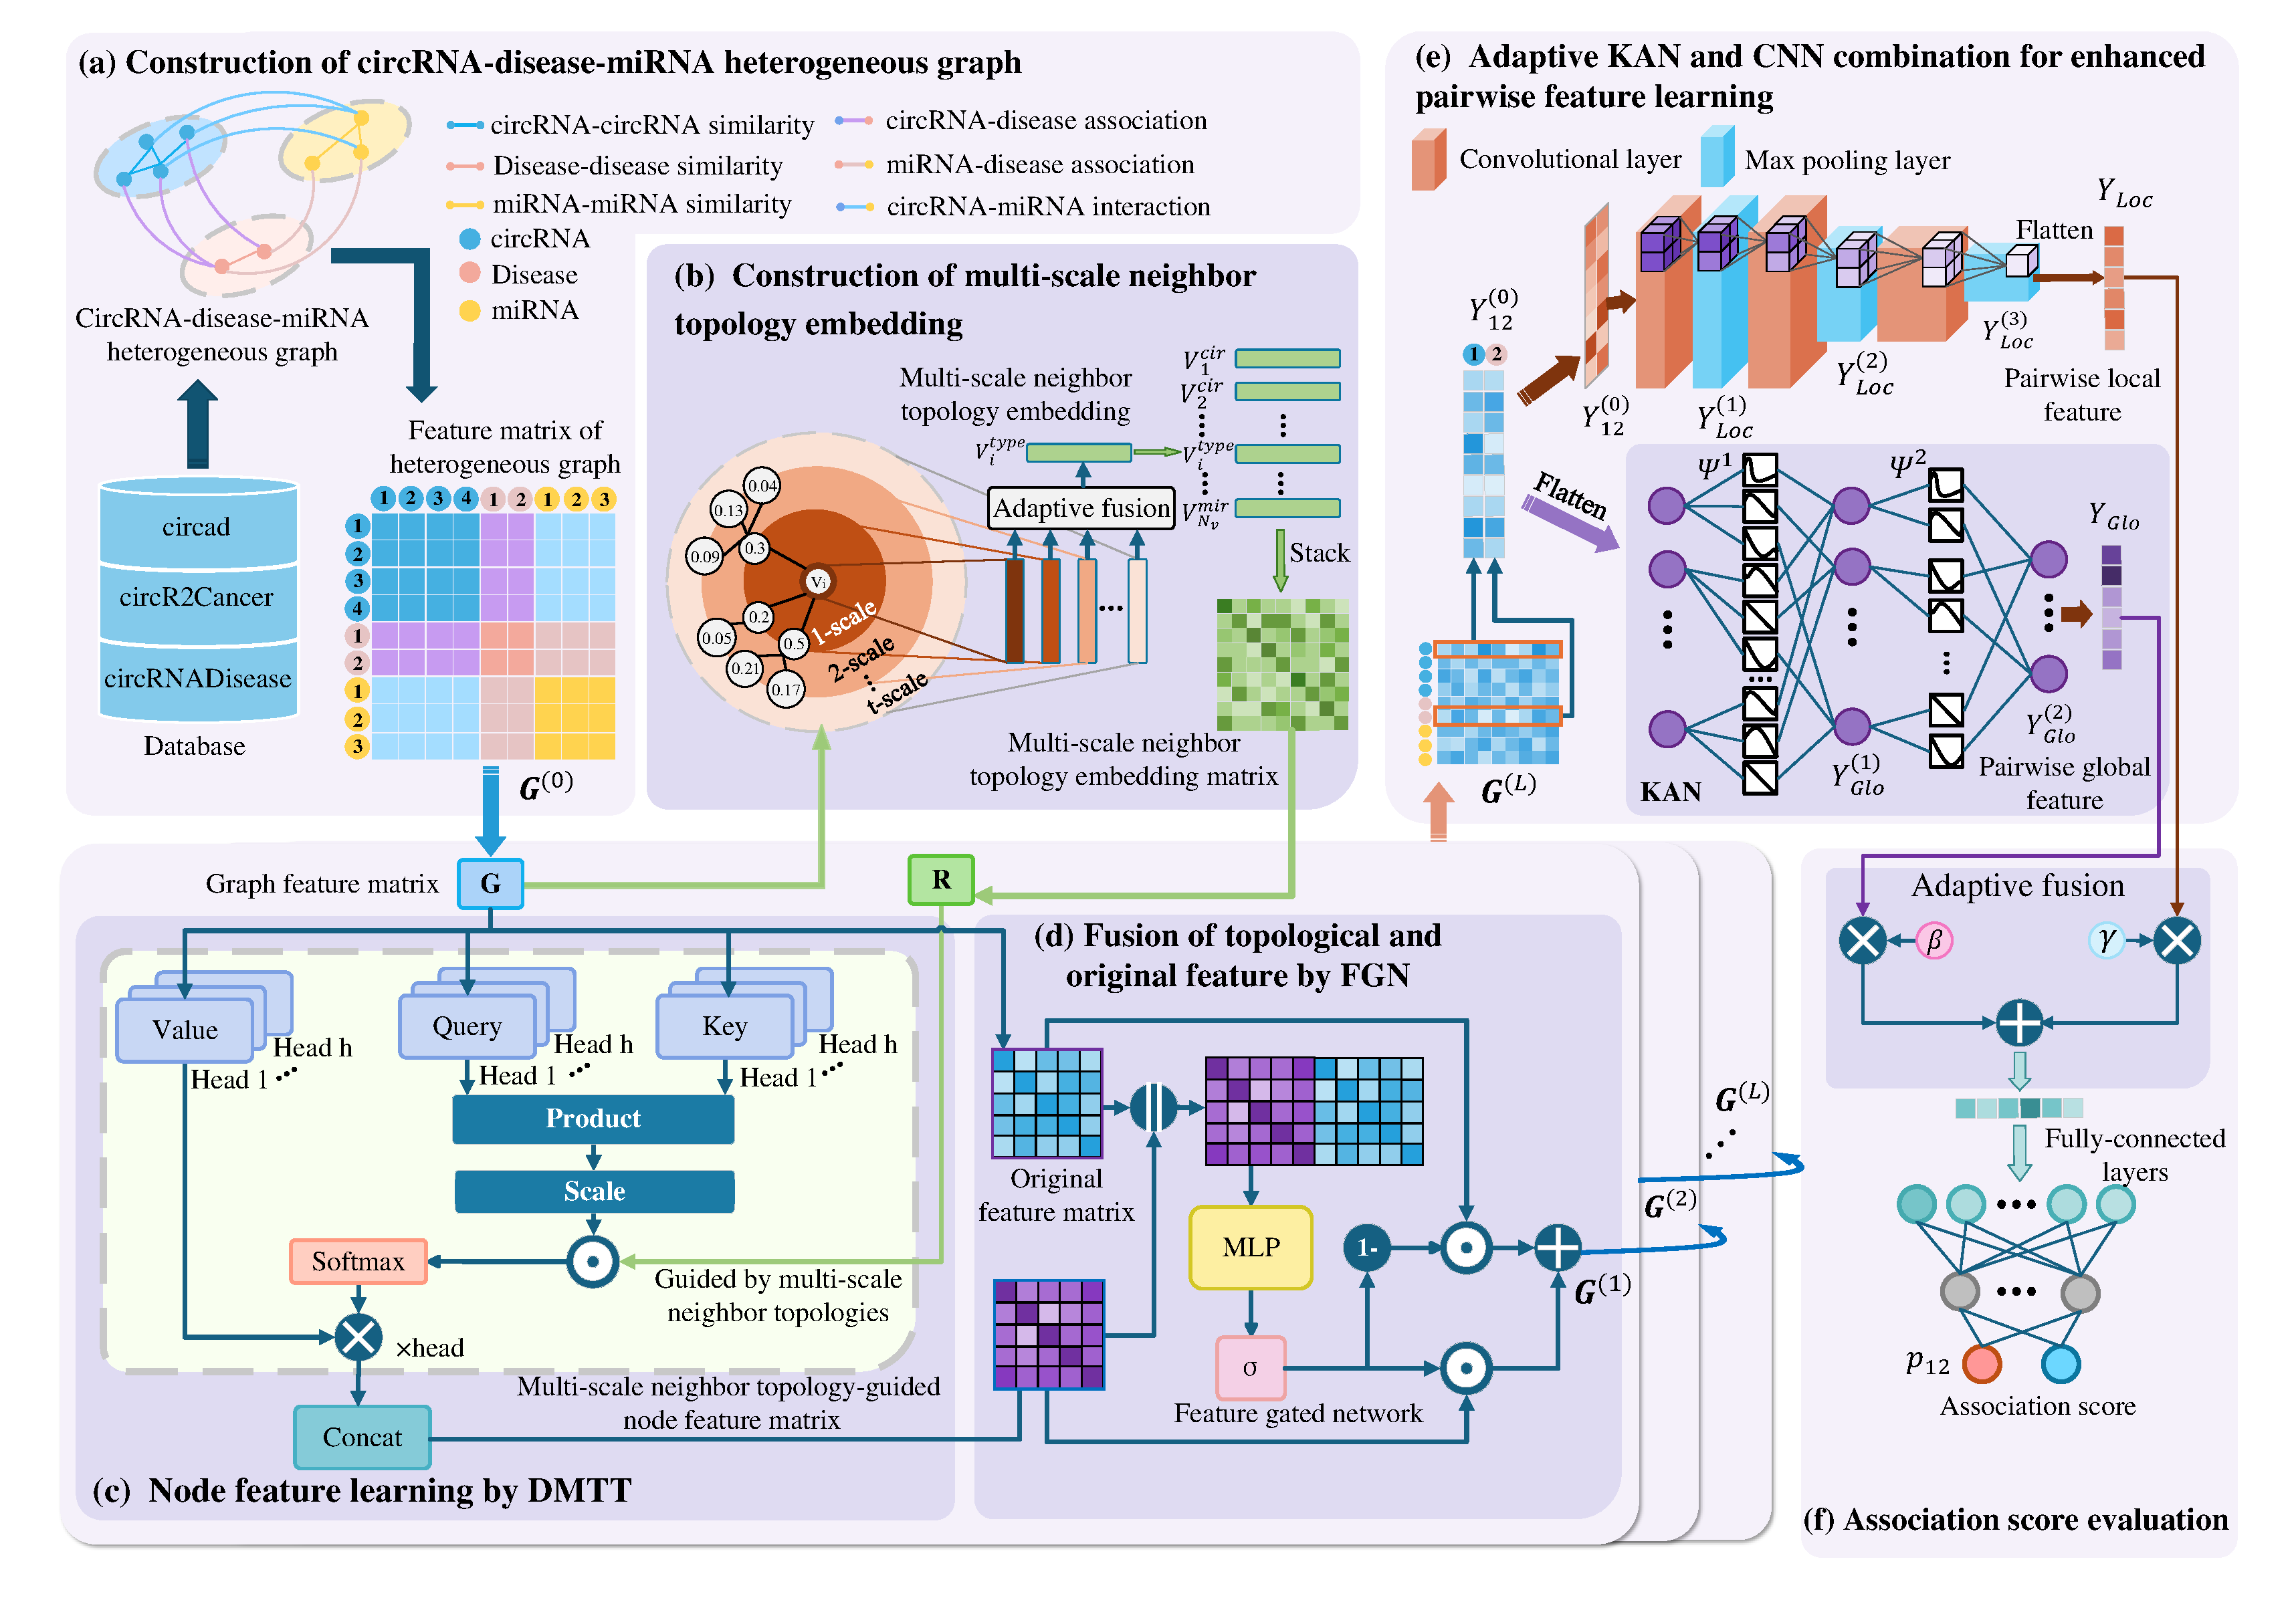
\includegraphics[width=8in]{fig/visio1.pdf}\\
	\vspace{0.2cm}
	\caption{\textcolor{blue}{The overall framework of MKCD. (a) Construction of the circRNA-disease-miRNA heterogeneous graph. (b) Building multi-scale neighbor topology embeddings through ARWR. (c) Learning the complex relationships among circRNA, miRNA, and disease nodes based on DMTT. (d) Fusion of topological features and original node features by FGN. (e) Learning local and global dependencies of node pair features based on ACK. (f) Adaptive fusion of the two representations to estimate circRNA-disease association scores.}}
	\label{fig:visio1}
	\vspace{0.1cm}
\end{figure*}

%---------------------------------------------------------------------------------------------------------------------


\section{Materials and methods}
\textcolor{blue}{We proposed a novel method, named as MKCD(Figure \ref{fig:visio1}), to predict circRNA-disease associations.}


\subsection{Dataset}
The dataset utilized in this study is derived from previous work \cite{lan2022kgancda}, which comprises two datasets containing circRNA and disease information. The first dataset covers 514 circRNAs, 62 diseases, and 564 miRNAs. The second dataset contains associations and interactions among 330 circRNAs, 79 diseases, and 245 miRNAs. We integrated these two datasets to form a new, larger dataset. This consolidated dataset consists of 989 circRNA-disease associations, 837 miRNA-disease associations, and 902 circRNA-miRNA interactions, covering a total of 834 circRNAs, 138 diseases, and 555 miRNAs. The original associations between circRNAs and diseases are obtained from the circR2Cancer database \cite{lan2020circr2cancer}, the circad database \cite{rophina2020circad}, and the circRNADisease database \cite{zhao2018circrna}.

\begin{figure*}[t]
	\centering
	% requires \usepackage{graphicx}
	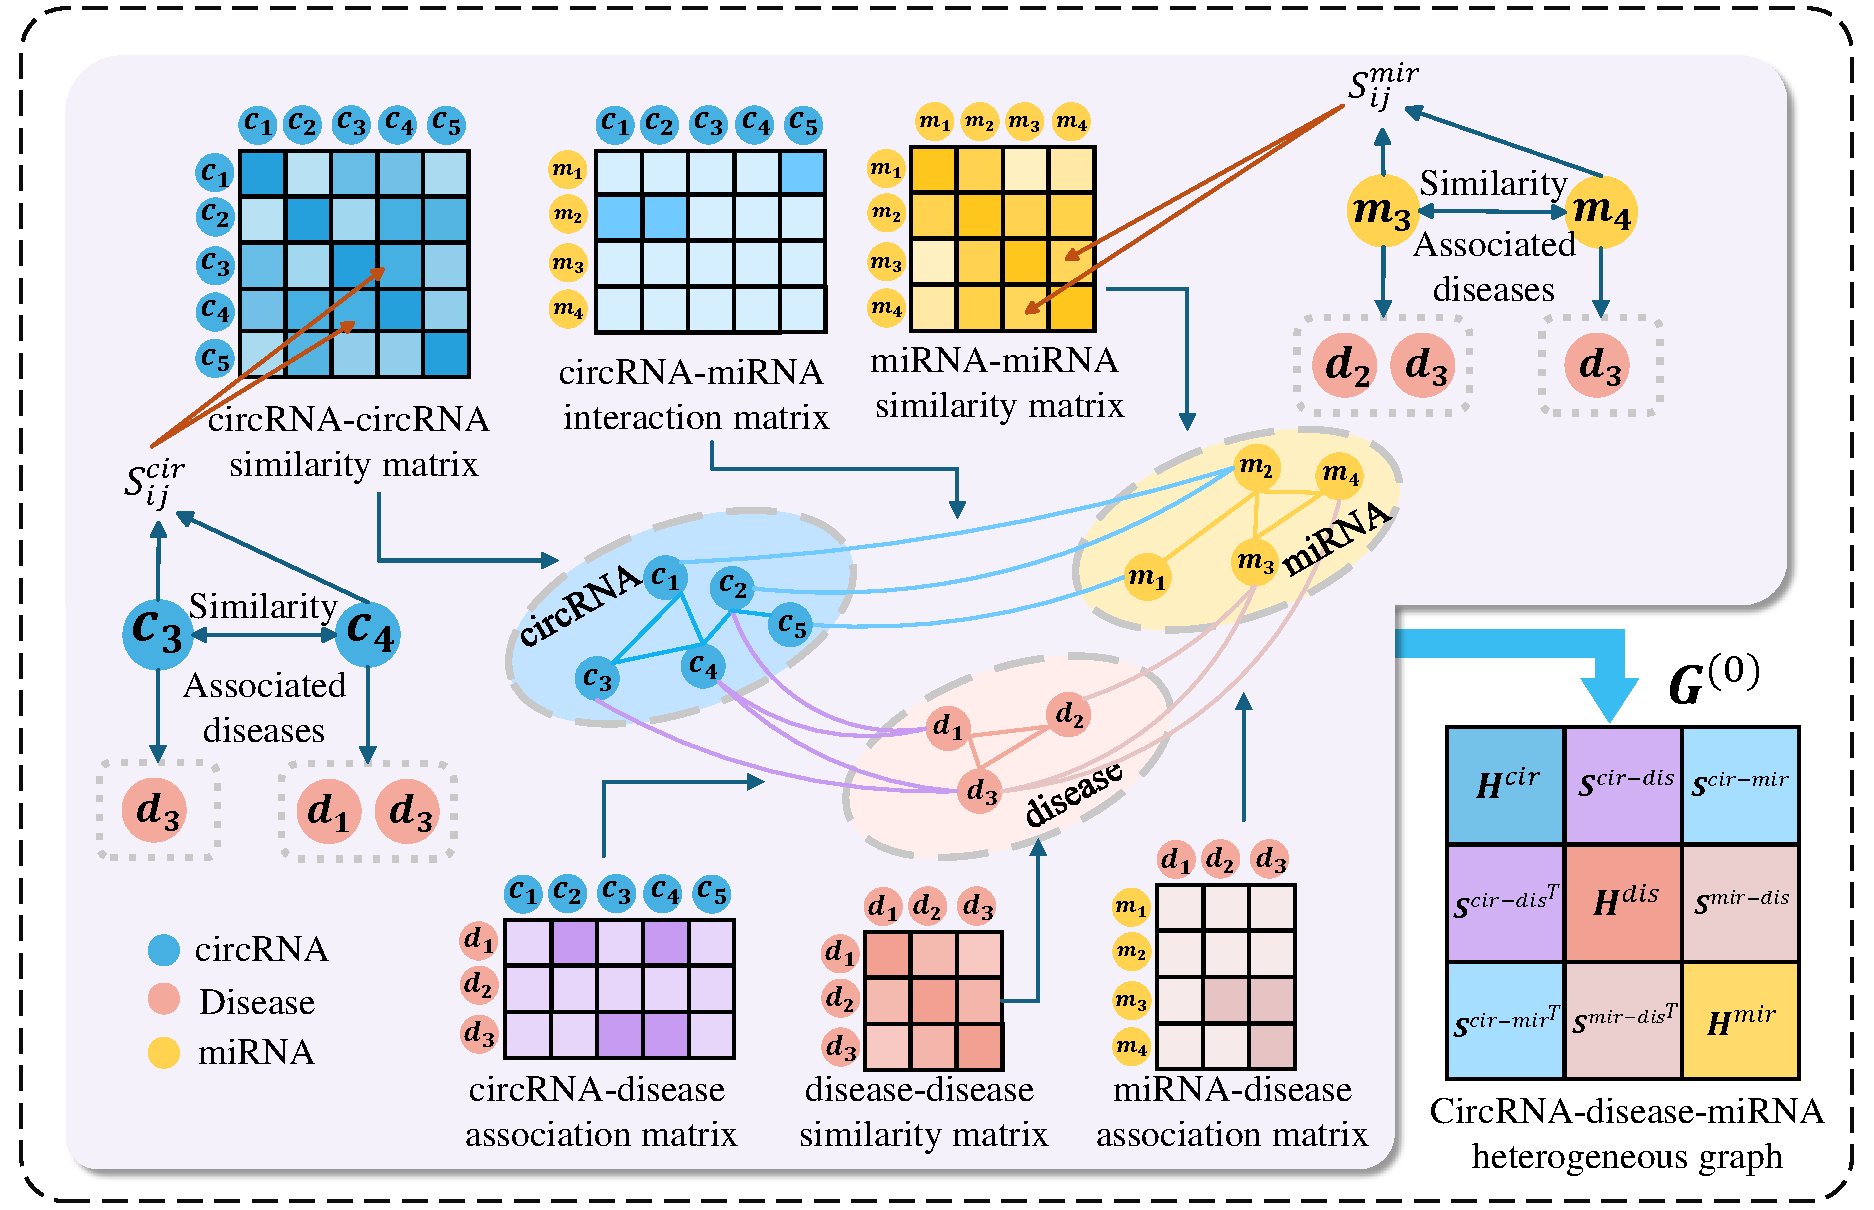
\includegraphics[width=7in]{fig/visio2.pdf}\\
	\vspace{0.2cm}
	\caption{\textcolor{blue}{Construction of the circRNA-disease-miRNA heterogeneous graph based on multi-source data.}}
	\label{fig:visio2}
	\vspace{0.1cm}
\end{figure*}


\subsection{CircRNA-disease-miRNA heterogeneous graph}
We constructed a three-layer heterogeneous graph $\mathcal{G}=(\mathcal{V}, \mathcal{E})$ using associations, interactions, and similarities among circRNAs, miRNAs, and diseases (Figure \ref{fig:visio2}). The node set $\mathcal{V}=\{V^{cir}\cup V^{dis}\cup V^{mir}\}$ comprises the set of circRNA nodes $V^{cir}$, disease nodes set $V^{dis}$, and miRNA nodes set $V^{mir}$. An edge $e_{ij} \in \mathcal{E}$ connects a pair of nodes $v_i,v_j \in \mathcal{V}$, represented by the association and interaction matrix $H$ and similarity matrix $S$.

The association and interaction matrix $H$ related to circRNAs, miRNAs, and diseases is defined as follows,
\begin{equation}
H = \left\{ \begin{array}{l}
{H^{cir-dis}} \in {\mathbbm{R}^{N_{cir}\times N_{dis}}}, \text{ if } {v_i} \in {V^{cir}}, {v_j} \in {V^{dis}};\\[5pt]
{H^{mir-dis}} \in {\mathbbm{R}^{N_{mir}\times N_{dis}}}, \text{ if } {v_i} \in {V^{mir}}, {v_j} \in {V^{dis}};\\[5pt]
{H^{cir-mir}} \in {\mathbbm{R}^{N_{cir}\times N_{mir}}}, \text{ if } {v_i} \in {V^{cir}}, {v_j} \in {V^{mir}};\\
\end{array} \right.
\end{equation}
where $H^{cir-dis}$, $H^{mir-dis}$, and $H^{cir-mir}$ denote the circRNA-disease association matrix, miRNA-disease association matrix, and circRNA-miRNA interaction matrix, respectively. $N_{cir}$, $N_{dis}$, and $N_{mir}$ represent the number of circRNAs, diseases, and miRNAs in the dataset. 
$H_{ij} \in H^{cir-dis} (H^{mir-dis})$ represents the association between the circRNA (miRNA) node $v_i^{cir}(v_i^{mir})$ and the disease node $v_j^{dis}$. For a circRNA (miRNA) node $v_i^{cir}$ ($v_i^{mir}$) and a disease node $d_j^{dis}$, if $H_{ij}^{cir-dis}=1$ ($H_{ij}^{mir-dis}=1$), it indicates the existence of an association between them; conversely, $H_{ij}^{cir-dis}=0$ ($H_{ij}^{mir-dis}=0$), no association has been observed. If $H_{ij}^{cir-mir}=1$, an interaction is present between the circRNA node $v_i^{cir}$ and the miRNA node $v_j^{mir}$; otherwise, $H_{ij}^{cir-mir}=0$.

$S$ represents the similarity matrices related to circRNAs, miRNAs, and diseases,
\begin{equation}
S = \left\{ \begin{array}{l}
{S^{cir}} \in {\mathbbm{R}^{N_{cir}\times N_{cir}}}, \text{ if } {v_i},{v_j} \in {V^{cir}};\\[5pt]
{S^{dis}} \in {\mathbbm{R}^{N_{dis}\times N_{dis}}}, \text{ if } {v_i},{v_j} \in {V^{dis}};\\[5pt]
{S^{mir}} \in {\mathbbm{R}^{N_{mir}\times N_{mir}}}, \text{ if } {v_i},{v_j} \in {V^{mir}};\\
\end{array} \right.
\end{equation}
where $S^{cir}$, $S^{dis}$, and $S^{mir}$ are the similarity matrices for circRNAs, diseases, and miRNAs, respectively. The values in $S^{cir}$, $S^{dis}$, and $S^{mir}$ range from 0 to 1, reflecting similarity between two nodes of the same type, with higher values indicating greater similarity.

According to the method proposed by Wang et al. \cite{wang2010inferring}, the similarity between two disease nodes $[v_i^{dis},v_j^{dis}]$ is calculated based on their directed acyclic graph (DAG). The similarities of circRNAs and miRNAs are calculated using the methods proposed by Wang et al. \cite{wang2010inferring} and Chen et al. \cite{chen2015constructing}, respectively, where the similarity of a pair of circRNAs (miRNAs) is derived from the similarity between the two sets of diseases associated with them. For instance, suppose the $i$-th circRNA node $v_i^{cir}$ is associated with $N_{cir}^i$ diseases, which forms the set $\Omega_i^{cir} = \{d_{ik} | k = 1, \ldots, N_{cir}^i\}$, and the $j$-th circRNA node $v_j^{cir}$ is associated with the disease set $\Omega_j^{cir} = \{d_{jl} | l = 1, \ldots, N_{cir}^j\}$. The similarity $S_{ij}^{cir}$ of $[v_i^{cir},v_j^{cir}]$ is determined by assessing the similarity between $\Omega_i^{cir}$ and $\Omega_j^{cir}$. Similarly, we can calculate the similarity $S_{ij}^{mir}$ for $[v_i^{mir},v_j^{mir}]$.

Based on the constructed association (interaction) matrix $H$ and the similarity matrix $S$, the original feature matrix of the heterogeneous graph $G^{(0)} \in \mathbb{R}^{N_v\times N_v}$ is defined as follows,
\begin{equation}
G^{(0)} = \left[\ \begin{array}{lll}
H^{cir} & S^{cir-dis} & S^{cir-mir}\\
{S^{cir-dis}}^T & H^{dis} & {S^{mir-dis}}^T\\
{S^{cir-mir}}^T & S^{mir-dis} & H^{mir}\\
\end{array} \right],
\end{equation}
where $N_v$ denotes the total number of circRNAs, miRNAs, and diseases, and ${S^{cir-dis}}^T$ represents the transpose of the matrix $S^{cir-dis}$. The $i$-th row $g_i$ of the matrix $G^{(0)}$ represents the node embedding of node $v_i \in \mathcal{V}$, which contains the associations and similarities involving $v_i$ and all circRNAs, diseases, and miRNAs. The set $\{g_i | 0 \leqslant i < N_{cir}\}$ denotes the collection of node embeddings for all circRNAs. Furthermore, the sets $\{g_i | N_{cir} \leqslant i < N_{cir} + N_{dis}\}$ and $\{g_i | N_{cir} + N_{dis} \leqslant i < N_{cir} + N_{dis} + N_{mir}\}$ represent the collections of node embeddings for all diseases and miRNAs, respectively.

\vspace{0.3cm}


\subsection{Construction of multi-scale neighbor topology embedding}
In the circRNA-disease-miRNA heterogeneous graph, the node $v_i$ has one-scale neighbors that can be reached in one step, or $d$-scale neighbors that can be reached in $d\ (d > 1)$ steps. The multi-scale topological structure formed by these neighboring nodes can provide important auxiliary information for predicting the associations between circRNAs and diseases. The contributions of low-scale (one-scale) neighbors and high-scale ($d$-scale) neighbors to the features learned for each node are different; thus, we employ ARWR (adaptive random walk with restart) to establish multi-scale neighbor topology embeddings (Figure \ref{fig:visio3}). Taking $v_i$ as an example, the walker starts from $v_i$ and performs random walks to travel to other nodes in the circRNA-disease-miRNA heterogeneous graph. The probability distribution of reaching all circRNA, disease, and miRNA nodes at time $t$ is given by $\theta _i{(t)} \in \mathbb{R}^{1 \times N_v}$,
\begin{equation}
\theta _i{(t)} = (1 - \lambda) O^T \theta _i{(t-1)} + \lambda \theta _i{(0)},
\label{eq:eq4}
\end{equation}
where the $j$-th value of $\theta _i{(t)}$ denotes the probability that the walker starts from $v_i$ reaches node $v_j$ after $t$ steps $(0 \leqslant j < N_v)$. $\theta _i{(0)}$ is the initial one-hot vector, where the $i$-th position is 1 and all other positions are 0. $\lambda$ is the probability that the walker restarts from the starting point; a larger value of $\lambda$ results in a smaller movement range of the walker within the network. $O \in \mathbb{R}^{N_v \times N_v}$ is obtained from the row-normalized matrix of $G^{(0)}$, where $o_{ij} \in O$ represents the probability of the walker traveling from $v_i$ to node $v_j$. $\theta _i{(t)}$ can be viewed as the probability distribution of reaching various nodes after $t$ steps from $v_i$, thus it serves as the $t$-scale neighbor topology embedding of $v_i$.

According to Eq.(\ref{eq:eq4}), we can build neighbor topology embeddings from scale 0 to scale $t$. These scale neighbor topology embeddings are adaptively fused to obtain the multi-scale neighbor topology embedding $\theta _i$ for $v_i$,
\begin{equation}
\theta _i = \eta_0  \theta _i{(0)} + \eta_1 \theta _i{(1)} + \cdots + \eta_k \theta _i{(k)} + \cdots + \eta_t \theta _i{(t)},
\end{equation}
where $\eta_k \in (0, 1)$ are randomly initialized learnable parameters, and $\sum_{k=0}^{t}\eta_k = 1$.

\begin{figure}[t]
	\centering
	% requires \usepackage{graphicx}
	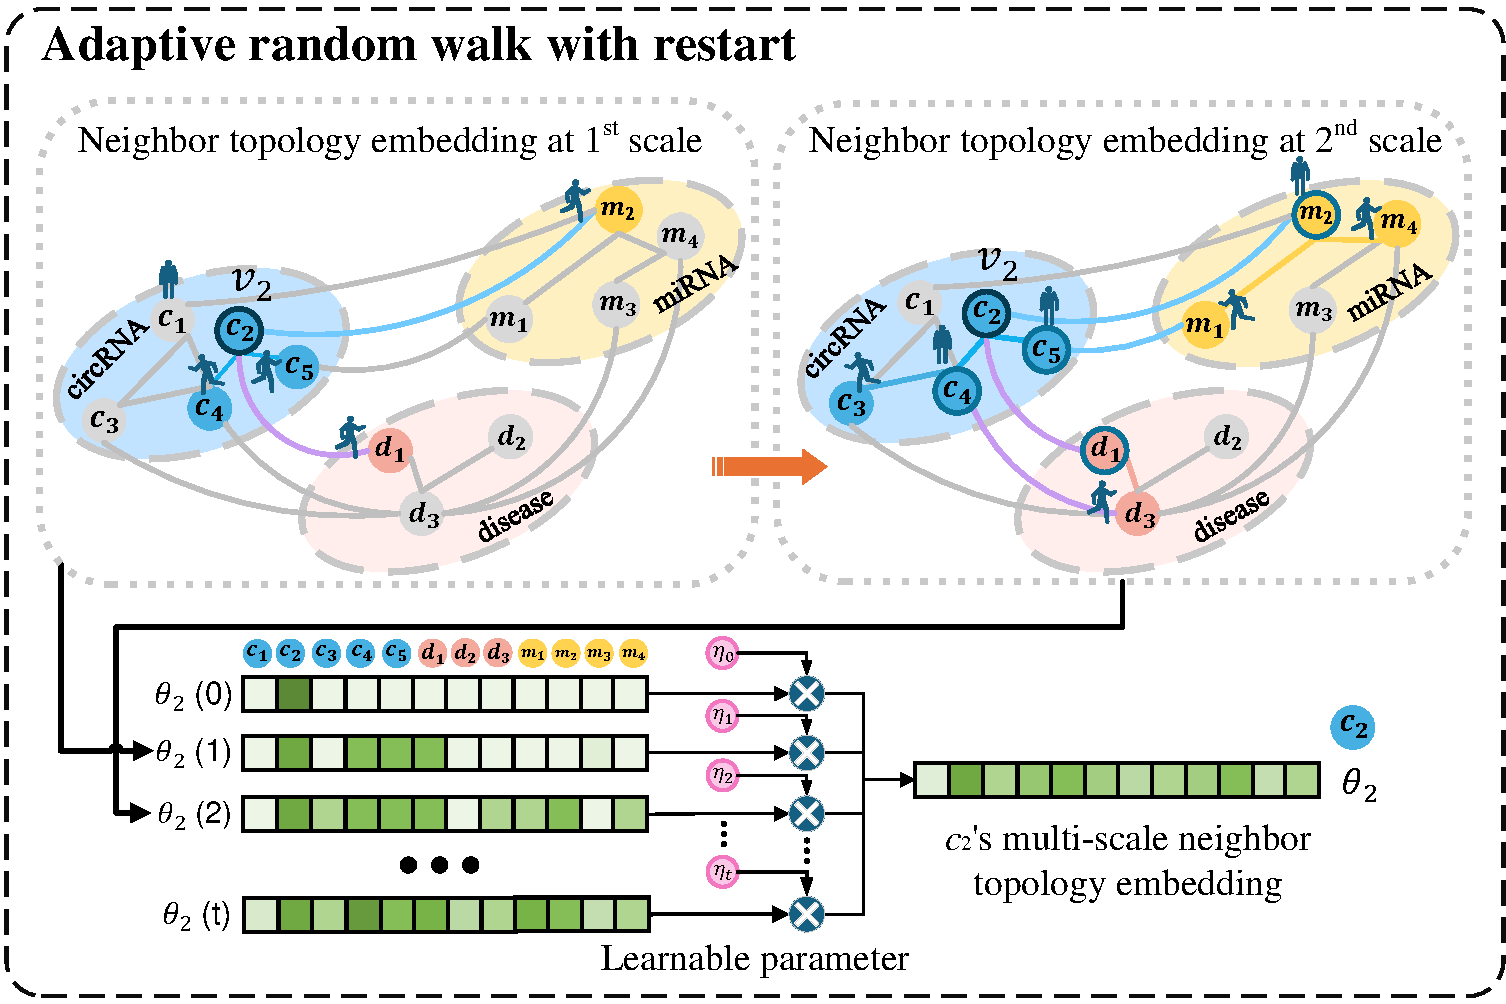
\includegraphics[width=4in]{fig/visio3.pdf}\\
	\vspace{0.2cm}
	\caption{\textcolor{blue}{Illustration of multi-scale neighbor topology embeddings constructed based on ARWR.}}
	\label{fig:visio3}
	\vspace{0.1cm}
\end{figure}

After applying the ARWR for each $v_i(0 \leqslant i < N_v)$, we can obtain the multi-scale neighbor embedding for all nodes . The multi-scale neighbor topology embeddings of all nodes are stacked vertically to form the embedding matrix $R \in \mathbb{R}^{N_v \times N_v}$,
\begin{equation}
	R = \left[\begin{array}{cccc}
		\theta _0\\
		\theta _1\\
		\vdots\\
		\theta _{N_v-1}
	\end{array}\right].
\end{equation}

\vspace{0.3cm}


\subsection{Node feature learning based on DMTT}
Typically, multiple circRNAs and miRNAs form interactions and collaboratively participate in the processes of various diseases. Therefore, there are close relationships among the features of multiple circRNAs, miRNAs, and disease nodes, making it necessary to establish a self-attention mechanism to capture these relationships. Traditional transformer focus solely on the similarities between node features and do not fully exploit the topological structures formed between nodes, especially the multi-scale neighbor topological structures. Inspired by the Transformer proposed by Vaswani et al. \cite{vaswani2017attention}, we introduce a DMTT (dynamic multi-scale neighbor topology-guided transformer) mechanism that utilizes the multi-scale neighbor topology embeddings established by ARWR to guide the learning of attention scores.

We incorporate a multi-head attention mechanism to overcome the problem of single-head attention easily falling into local optima during the training process, thereby reducing bias in the learning process. For the $m$-th attention head, we first establish the query matrix $Q_{m}^{(l)} \in \mathbb{R}^{N_v \times \frac{N_v}{h}}$, the key matrix $K_{m}^{(l)} \in \mathbb{R}^{N_v \times \frac{N_v}{h}}$, and the value matrix $V_{m}^{(l)} \in \mathbb{R}^{N_v \times \frac{N_v}{h}}$ as follows,
\begin{equation}
	\begin{aligned}
		{Q_{m}^{(l)}} &= G^{{(l - 1)}}{W_{m}^{Q{(l)}}} \\
		{K_{m}^{(l)}} &= G^{{(l - 1)}}{W_{m}^{K{(l)}}} ,\\
		{V_{m}^{(l)}} &= G^{(l - 1)}{W_{m}^{V{(l)}}}
	\end{aligned}
\end{equation}
where $G^{(l - 1)} \in \mathbb{R}^{N_v \times N_v}$ is the feature matrix of the graph nodes at layer $l$ $(1 \leqslant l \leqslant L)$. When $l = 1$, $G^{(0)}$ represents the original feature matrix, and $h$ is the number of attention heads. $Q_{m}^{(l)}$, $K_{m}^{(l)}$, and $V_{m}^{(l)}$ are obtained from $G^{(l - 1)}$ through different linear projections, with $W_{m}^{Q{(l)}}$, $W_{m}^{K{(l)}}$, and $W_{m}^{V(l)} \in \mathbb{R}^{N_v \times \frac{N_v}{h}}$ being the corresponding weight matrices for the linear projections. Then, we perform a dot product operation on $Q_{m}^{(l)}$ and ${K_{m}^{(l)}}^T$ to obtain the attention score matrix ${S_{m}^{(l)}} \in \mathbb{R}^{N_v \times N_v}$,
\begin{equation}
	{S_{m}^{(l)}} = \frac{Q_{m}^{(l)}{K_{m}^{(l)}}^T}{\sqrt{d}},
\end{equation}
where $d = \frac{N_v}{h}$ and $\sqrt{d}$ is a scaling factor used to adjust the magnitude of the attention scores to enhance numerical stability during the training process. The $i$-th row of $S_{m}^{(l)}$ records the attention scores from all circRNA, disease, and miRNA nodes to $v_i$.

After the $(l-1)$-th layer DMTT, the topology among the nodes changes, and a new multi-scale neighbor topology embedding $R^{(l)}$ for each node is reconstructed through ARWR based on $G^{(l - 1)}$. The $i$-th row of $R^{(l)}$ records the neighbor topology of $v_i$ with all other circRNA, disease, and miRNA nodes after the $(l-1)$-th layer self-attention encoding. We perform a Hadamard product operation between the $i$-th row of $R^{(l)}$ and the $i$-th row of $S_{m}^{(l)}$. This approach allows the multi-scale neighbor topology embeddings to guide the learning of attention scores. We establish the multi-scale neighbor topology-guided attention score matrix $\widetilde{S}_{m}^{(l)} \in \mathbb{R}^{N_v \times N_v}$ as follows,
\begin{equation}
	\widetilde{S}_{m}^{(l)} = S_{m}^{(l)} \odot R^{(l)},
\end{equation}
where $\odot$ denotes the Hadamard product operation. Multiplying $\widetilde{S}_{m}^{(l)}$ with $V_{m}^{(l)}$ produces the node features ${Z_{m}^{(l)}} \in \mathbb{R}^{N_v \times \frac{N_v}{h}}$ learned by the $m$-th attention head,
\begin{equation}
	{Z_{m}^{(l)}} = softmax(\widetilde{S}_{m}^{(l)})V_{m}^{(l)}.
\end{equation}
Finally, by concatenating the node features learned by the $h$ attention heads, we obtain the multi-scale neighbor topology-guided node feature matrix $\hat{G}^{(l)} \in \mathbb{R}^{N_v \times N_v}$ for layer $l$,
\begin{equation}
	\hat{G}^{(l)}= \bigg\|_{\substack{i\in {[1,h]}}} Z^{(l)}_{m},
\end{equation}
where $\|$ denotes the concatenation operation. The $i$-th row of $\hat{G}^{(l)}$ records the features of $v_i$ learned at layer $l$.

\vspace{0.3cm}


\subsection{Fusion of multiple types of features based on FGN}
In DMTT, the feature matrix ${G}^{(l - 1)}$ that is input at layer $l$ contains more detailed information about each node, while the feature matrix $\hat{G}^{(l)}$ learned based on DMTT places greater emphasis on the information guided by multi-scale neighbor topology embedding. Therefore, it is necessary to incorporate ${G}^{(l - 1)}$ into the feature learning process at layer $l$. To integrate the information contained in $\hat{G}^{(l)}$ and $G^{(l - 1)}$, we establish a FGN (feature gate network) in DMTT at layer $l$, with the weight matrix denoted as $\alpha^{(l)}$:
\begin{equation}
    \alpha^{(l)} = \sigma (W^{gate(l)}(\hat{G}^{(l)}\| G^{(l - 1)}) + b^{gate(l)}),
\end{equation}
where $W^{gate(l)}$ and $b^{gate(l)}$ are learnable weight matrices and bias, and $\sigma$ is the Sigmoid activation function. All parameters of the FGN are randomly initialized and are learnable during the training process, allowing it to discern the more significant features in $\hat{G}^{(l)}$ and $G^{(l - 1)}$.

The FGN-enhanced node feature representation is denoted as ${G}^{(l)} \in \mathbb{R}^{N_v \times N_v}$:
\begin{equation}
    {G}^{(l)} =  \alpha^{(l)} \odot \hat{G}^{(l)} + (1 - \alpha^{(l)}) \odot G^{(l - 1)}.
\end{equation}
When $l \neq L$, $G^{(l)}$ will serve as the input for the next layer of DMTT, where $l = L$, $G^{(L)}$ represents the final node feature representation matrix.

\vspace{0.3cm}


\subsection{Adaptive KAN and CNN combination enhanced pairwise feature learning}
If the circRNA node $v_i^{cir}$ and the disease node $d_j^{dis}$ have similarities, associations, or interactions with the same circRNAs, diseases, and miRNAs, then the node pair $[v_i^{cir}, d_j^{dis}]$ is more likely to be associated. Based on this biological premise, we vertically stack the feature representations obtained from the FGN-enhanced DMTT for both circRNA and disease nodes, forming a node pair-level feature representation ${Y_{ij}^{(0)}} \in \mathbb{R}^{2 \times N_v}$,
\begin{equation}
    {Y_{ij}^{(0)}} = \begin{bmatrix} {G^{(L)}_i} \\ {G^{(L)}_j} \end{bmatrix},
\end{equation}
where the sets $\{G^{(L)}_{i} | 0 \leqslant i < N_{cir}\}$ and $\{G^{(L)}_j | N_{cir} \leqslant j < N_{cir} + N_{dis}\}$ represent the node feature representations of all circRNAs and diseases in $G^{(L)}$, respectively.

The ACK (adaptive KAN and CNN combination learning) we designed will further extract the information within the circRNA-disease node pairs. The KAN module we established learns the paired node representations from a global perspective, while the CNN module focuses more on extracting local information of the paired node representations.

\vspace{0.3cm}

\subsubsection{Pairwise global feature learning based on KAN}
Compared to the multi-layer perceptron (MLP), KAN replaces weight parameters and activation functions with learnable functions to adaptively learn the weights of the connections between neurons. This learnable function is typically composed of multiple stacked spline functions, enabling the KAN network to better capture the complex relationships among the features in ${Y_{ij}^{(0)}}$. Through multiple layers of the KAN network, a feature representation of the node pair $[v_i^{cir}, d_j^{dis}]$ is learned from a global perspective. The input feature representation of the node pair at the $l$-th layer $Y_{Glo}^{(l - 1)}$ is transformed into the pairwise global feature representation ${Y}_{Glo}^{(l)}$ after passing through the $l$-th layer of the global feature learning module based on the KAN network,
\begin{equation}
    {Y}_{Glo}^{(l)} = KAN^{(l)}(Y_{Glo}^{(l - 1)}) = \varPsi^{(l)}(Y_{Glo}^{(l - 1)}),
\end{equation}
where $KAN^{(l)}$ denotes the $l$-th KAN layer. When $l=1$, $Y_{Glo}^{(0)}$ represents the original circRNA-disease node pair-level feature representation $Y_{ij}^{(0)}$. When $l=L$, $Y_{Glo}^{(L)}$ represents the final pairwise global feature representation ${Y}_{Glo} \in \mathbb{R}^{1\times f}$, where $f$ is the feature dimension. The matrix $\varPsi^{(l)}$ is composed of learnable functions for the $l$-th KAN layer, containing a total of $n^{(l - 1)} \times n^{(l)}$ learnable functions. Therefore, $\varPsi^{(l)}$ is defined as,
\begin{equation}
    \varPsi^{(l)} = \left(
    \begin{array}{cccc}
        \psi_{1,1} & \psi_{1,2} & \cdots & \psi_{1,n^{(l-1)}} \\
        \psi_{2,1} & \psi_{2,2} & \cdots & \psi_{2,n^{(l-1)}} \\
        \vdots & \vdots & \ddots & \vdots \\
        \psi_{n^{(l)},1} & \psi_{n^{(l)},2} & \cdots & \psi_{n^{(l)},n^{(l-1)}}
    \end{array}
    \right),
\end{equation}
where $n^{(l - 1)}$ and $n^{(l)}$ represent the number of neurons in the $(l - 1)$-th and $l$-th layers, respectively. The $\psi_{i,j}$ corresponds to the learnable function of the edge connecting the $i$-th neuron in the $l$-th layer to the $j$-th neuron in the $(l - 1)$-th layer. The $\psi_{i,j}$ is composed of a basis function and a B-spline function,
\begin{equation}
    \psi_{i,j} = \omega_{b}b(x) + \omega_{s}spline(x),
\end{equation}
\begin{equation}
    spline(x) = \sum_{k = 1}^{n_{grid}}c_{k} B_{k},
\end{equation}
where $b(x)$ is the basis function ${SiLU}$, and $\omega_{b}$ and $\omega_{s}$ are learnable weight parameters. The B-spline function $spline(x)$ is obtained by stacking $n_{grid}$ B-spline basis functions $B_{k}$, where $c_{k}$ is the learnable parameter for each $B_{k}$.

\vspace{-0.3cm}

\subsubsection{Pairwise local feature learning based on CNN}
We have established a CNN module to learn the local features of circRNA-disease node pairs. In the CNN, each block consists of a convolution layer followed by a pooling layer. In the $l$-th block $(1 \leqslant l \leqslant D)$, given the feature representation of a circRNA-disease node pair ${Y}_{Loc}^{(l - 1)}$, we use the convolution and pooling operations to extract its pairwise local features ${Y}_{Loc}^{(l)}$,
\begin{equation}
{Y}_{Loc}^{(l)} = max(\mathop{\rm{\tau}}({W_{conv}^{(l)}}  * {Y}_{Loc}^{(l - 1)} + {b_{conv}^{(l)}})),
\end{equation}
where * denotes the convolution operation, $W_{conv}^{(l)}$ and $b_{conv}^{(l)}$ are the sets of convolution kernels and bias, respectively, $\tau$ is the Leaky ReLU activation function, and $max$ represents the max pooling operation. $Y_{Loc}^{(0)}$ is the original feature representation of the circRNA-disease node pair $Y_{ij}^{(0)}$. When $l = D$, the dimension of $Y_{Loc}^{(D)}$ is reduced and flattened to obtain the final pairwise local feature representation $Y_{Loc} \in \mathbb{R}^{1\times f}$.

\vspace{-0.4cm}

\subsubsection{Adaptive fusion of pairwise local features and global features}
The pairwise local feature representation ${Y_{Loc}}$ and global feature representation ${Y_{Glo}}$ hold varying degrees of importance for the feature representation learning of each circRNA (disease) node. We assign a learnable weight parameter $s_{\beta}$ for ${Y_{Glo}}$ and $s_{\gamma}$ for ${Y_{Loc}}$, and after normalization, we obtain $\beta$ and $\gamma$,
\begin{equation}
    \beta = \frac{e^{s_{\beta}}}{e^{s_{\beta}} + e^{s_{\gamma}}}\ , \quad \gamma = \frac{e^{s_{\gamma}}}{e^{s_{\beta}} + e^{s_{\gamma}}}\ .
\end{equation}
The final feature representation of the circRNA-disease node pair is defined as ${Y}_{F} \in \mathbb{R}^{1\times f}$,
\begin{equation}
    {Y}_{F} = \beta \cdot {Y_{Loc}} + \gamma \cdot {Y_{Glo}}\ \ ,
\end{equation}
where $\cdot$ denotes scalar multiplication.

\vspace{0.3cm}


\subsection{Association score evaluation and optimization}
We utilize a fully connected layer to derive the association prediction score vector $p_{ij} \in \mathbb{R}^{1\times 2}$ for the node pair $[v_i^{cir}, d_j^{dis}]$,
\begin{equation}
    p_{ij} = softmax(W_{Fin}Y_{F} + b_{Fin}),
\end{equation}
where $W_{Fin}$ and $b_{Fin}$ are the weight matrix and bias of the fully connected layer, respectively. The vector $p_{ij} = [p_{pos}, p_{neg}]$ represents the probabilities that $v_i^{cir}$ is associated with $d_j^{dis}$ or not, denoted as $p_{pos}$ and $p_{neg}$, respectively.

During the training process, we employ the AdamW algorithm and back propagation to optimize our model. We use the cross-entropy function to estimate the model's loss,
\begin{equation}
    loss = - \sum\limits_{(i,j) \in N} \left[ y_{ij} \log (p_{pos}) + (1 - y_{ij}) \log (p_{neg}) \right],
\end{equation}
where $N$ denotes the sample set of all circRNA-disease node pairs. $y_{ij}$ represents the true association label between the circRNA node $v_i^{cir}$ and the disease node $d_j^{dis}$. When there is an association between $v_i^{cir}$ and $d_j^{dis}$, $y_{ij} = 1$; otherwise, $y_{ij} = 0$.
%---------------------------------------------------------------------------------------------------------------------

\section{Experimental evaluations and discussions}	
\subsection{Parameter settings}
In the ARWR module, we utilize the 0 to 2-scale neighbor topology to construct multi-scale neighbor topology embeddings, with the restart probability $\lambda$ for random walks set to 0.7. For the DMTT module, the number of layers $L$ is set to 2, and in each layer of the DMTT, the number of attention heads $h$ is set to 4. In the pairwise local feature learning module, we employ three blocks, where the convolution kernel sizes of the first two blocks are $2\times 2$, and the convolution kernel of the third block is $1\times 2$. The pooling layer of the first block uses a window size of $2\times 2$, while the pooling windows for the remaining two blocks are both set to $1\times 7$. In the pairwise global feature learning module, we establish a 2-layer KAN network with the number of neurons set to 1024 and 256, respectively, and the number of $n_{grid}$ for the B-spline function is set to 5. We train MKCD using an Nvidia GeForce RTX 4060, utilizing the PyTorch framework and optimizing using the AdamW algorithm. The training process consisted of 40 epochs, with a batch size of 32, a learning rate of 0.001, and a weight decay of 0.0001.

\vspace{0.3cm}


\subsection{Evaluation metrics}
We employ five-fold cross-validation to evaluate the predictive performance of MKCD and other comparative methods. All known circRNA-disease associations are treated as positive samples and randomly divided into five equal parts, while all unobserved circRNA-disease associations are considered as negative samples. In each fold, we use four parts of positive samples and an equal number of randomly selected negative samples as the training set, while the remaining positive samples and all unselected negative samples constitute the test set.

We select the area under the receiver operating characteristic curve (AUC) \cite{hajian2013receiver} and the area under the precision-recall curve (AUPR) \cite{saito2015precision} as evaluation metrics. AUC and AUPR are calculated separately for each fold, and the averages of these five folds yields the final AUC and AUPR scores. Furthermore, considering that biologists typically choose candidates from the top of the ranked list for further validation, we calculate the recall rate of the top k disease-related circRNAs.

\vspace{0.3cm}


\subsection{Ablation experiments}
To validate the effectiveness of MARWR (multi-scale neighbor topology embedding based on adaptive random walk with restart), DMTT (dynamic multi-scale neighbor topology-guided transformer), FGN (feature gate network), and ACK (adaptive KAN and CNN combination learning), we conducted a series of ablation experiments (Table \ref{tab:tab1}). We sequentially removed the MARWR, DMTT, FGN, and ACK modules from MKCD and calculated the corresponding AUC and AUPR. We observed that when all modules were retained, the complete model MKCD achieved the best predictive performance, with AUC and AUPR values of 0.947 and 0.271, respectively. When the MARWR module was removed, the AUC and AUPR decreased by 3.4\% and 6.8\%, respectively, indicating that the introduction of multi-scale neighbor topology embedding plays a crucial role in enhancing the accuracy of circRNA and disease association predictions. The removal of DMTT and FGN resulted in a 3.8\% drop in AUC and a 7.6\% drop in AUPR, confirming the necessity of utilizing the multi-scale neighbor topology formed by circRNA, disease, and miRNA nodes to learn node feature representations. The complete model improved AUC and AUPR by 2.4\% and 5.0\%, respectively, compared to when FGN was ignored, suggesting that the incorporation of detailed features benefits the learning of node features. Finally, the removal of ACK led to a decrease of 1.6\% in AUC and 3.1\% in AUPR, demonstrating the effectiveness of the adaptive fusion of pairwise local features and global features in enhancing circRNA-disease association prediction performance.

The results of the ablation experiments indicate that DMTT contributes the most to circRNA-disease association prediction, primarily because DMTT encodes the relationships among multiple features of circRNA, disease, and miRNA nodes. MARWR contributes the second largest to the prediction results, as MARWR effectively introduces multi-scale neighbor topology embedding into node feature learning.

\begin{table}[!t]
	\label{tab:01}
    \centering
    \begin{threeparttable}[b]
        \vspace{0.4cm}
        \caption{Results of ablation experiments of MKCD.}\label{tab:tab1}
        \begin{tabular}{m{1.8cm}<{\centering}m{1.2cm}<{\centering}m{1.1cm}<{\centering}m{1.1cm}<{\centering}|m{1.2cm}<{\centering}m{1.5cm}<{\centering}}
            \hline
            \textbf{MARWR} &\textbf{DMTT} & \textbf{FGN} & \textbf{ACK} & \textbf{Average AUC} & \textbf{Average AUPR} \\
            \hline
            \ding{55} &\checkmark & \checkmark & \checkmark & 0.913 & 0.203 \\
            \checkmark &\ding{55} & \ding{55} & \checkmark & 0.909 & 0.195 \\
            \checkmark &\checkmark & \ding{55} & \checkmark & 0.923 & 0.221 \\
            \checkmark &\checkmark & \checkmark & \ding{55} & 0.931 & 0.240 \\
            \checkmark &\checkmark & \checkmark & \checkmark & \textbf{0.947} & \textbf{0.271} \\
            \hline
        \end{tabular}
    \end{threeparttable}
    \vspace{-0.4cm}
\end{table}

\vspace{0.3cm}


\subsection{Comparison with other methods}

\begin{figure*}[!t]
    \centering
    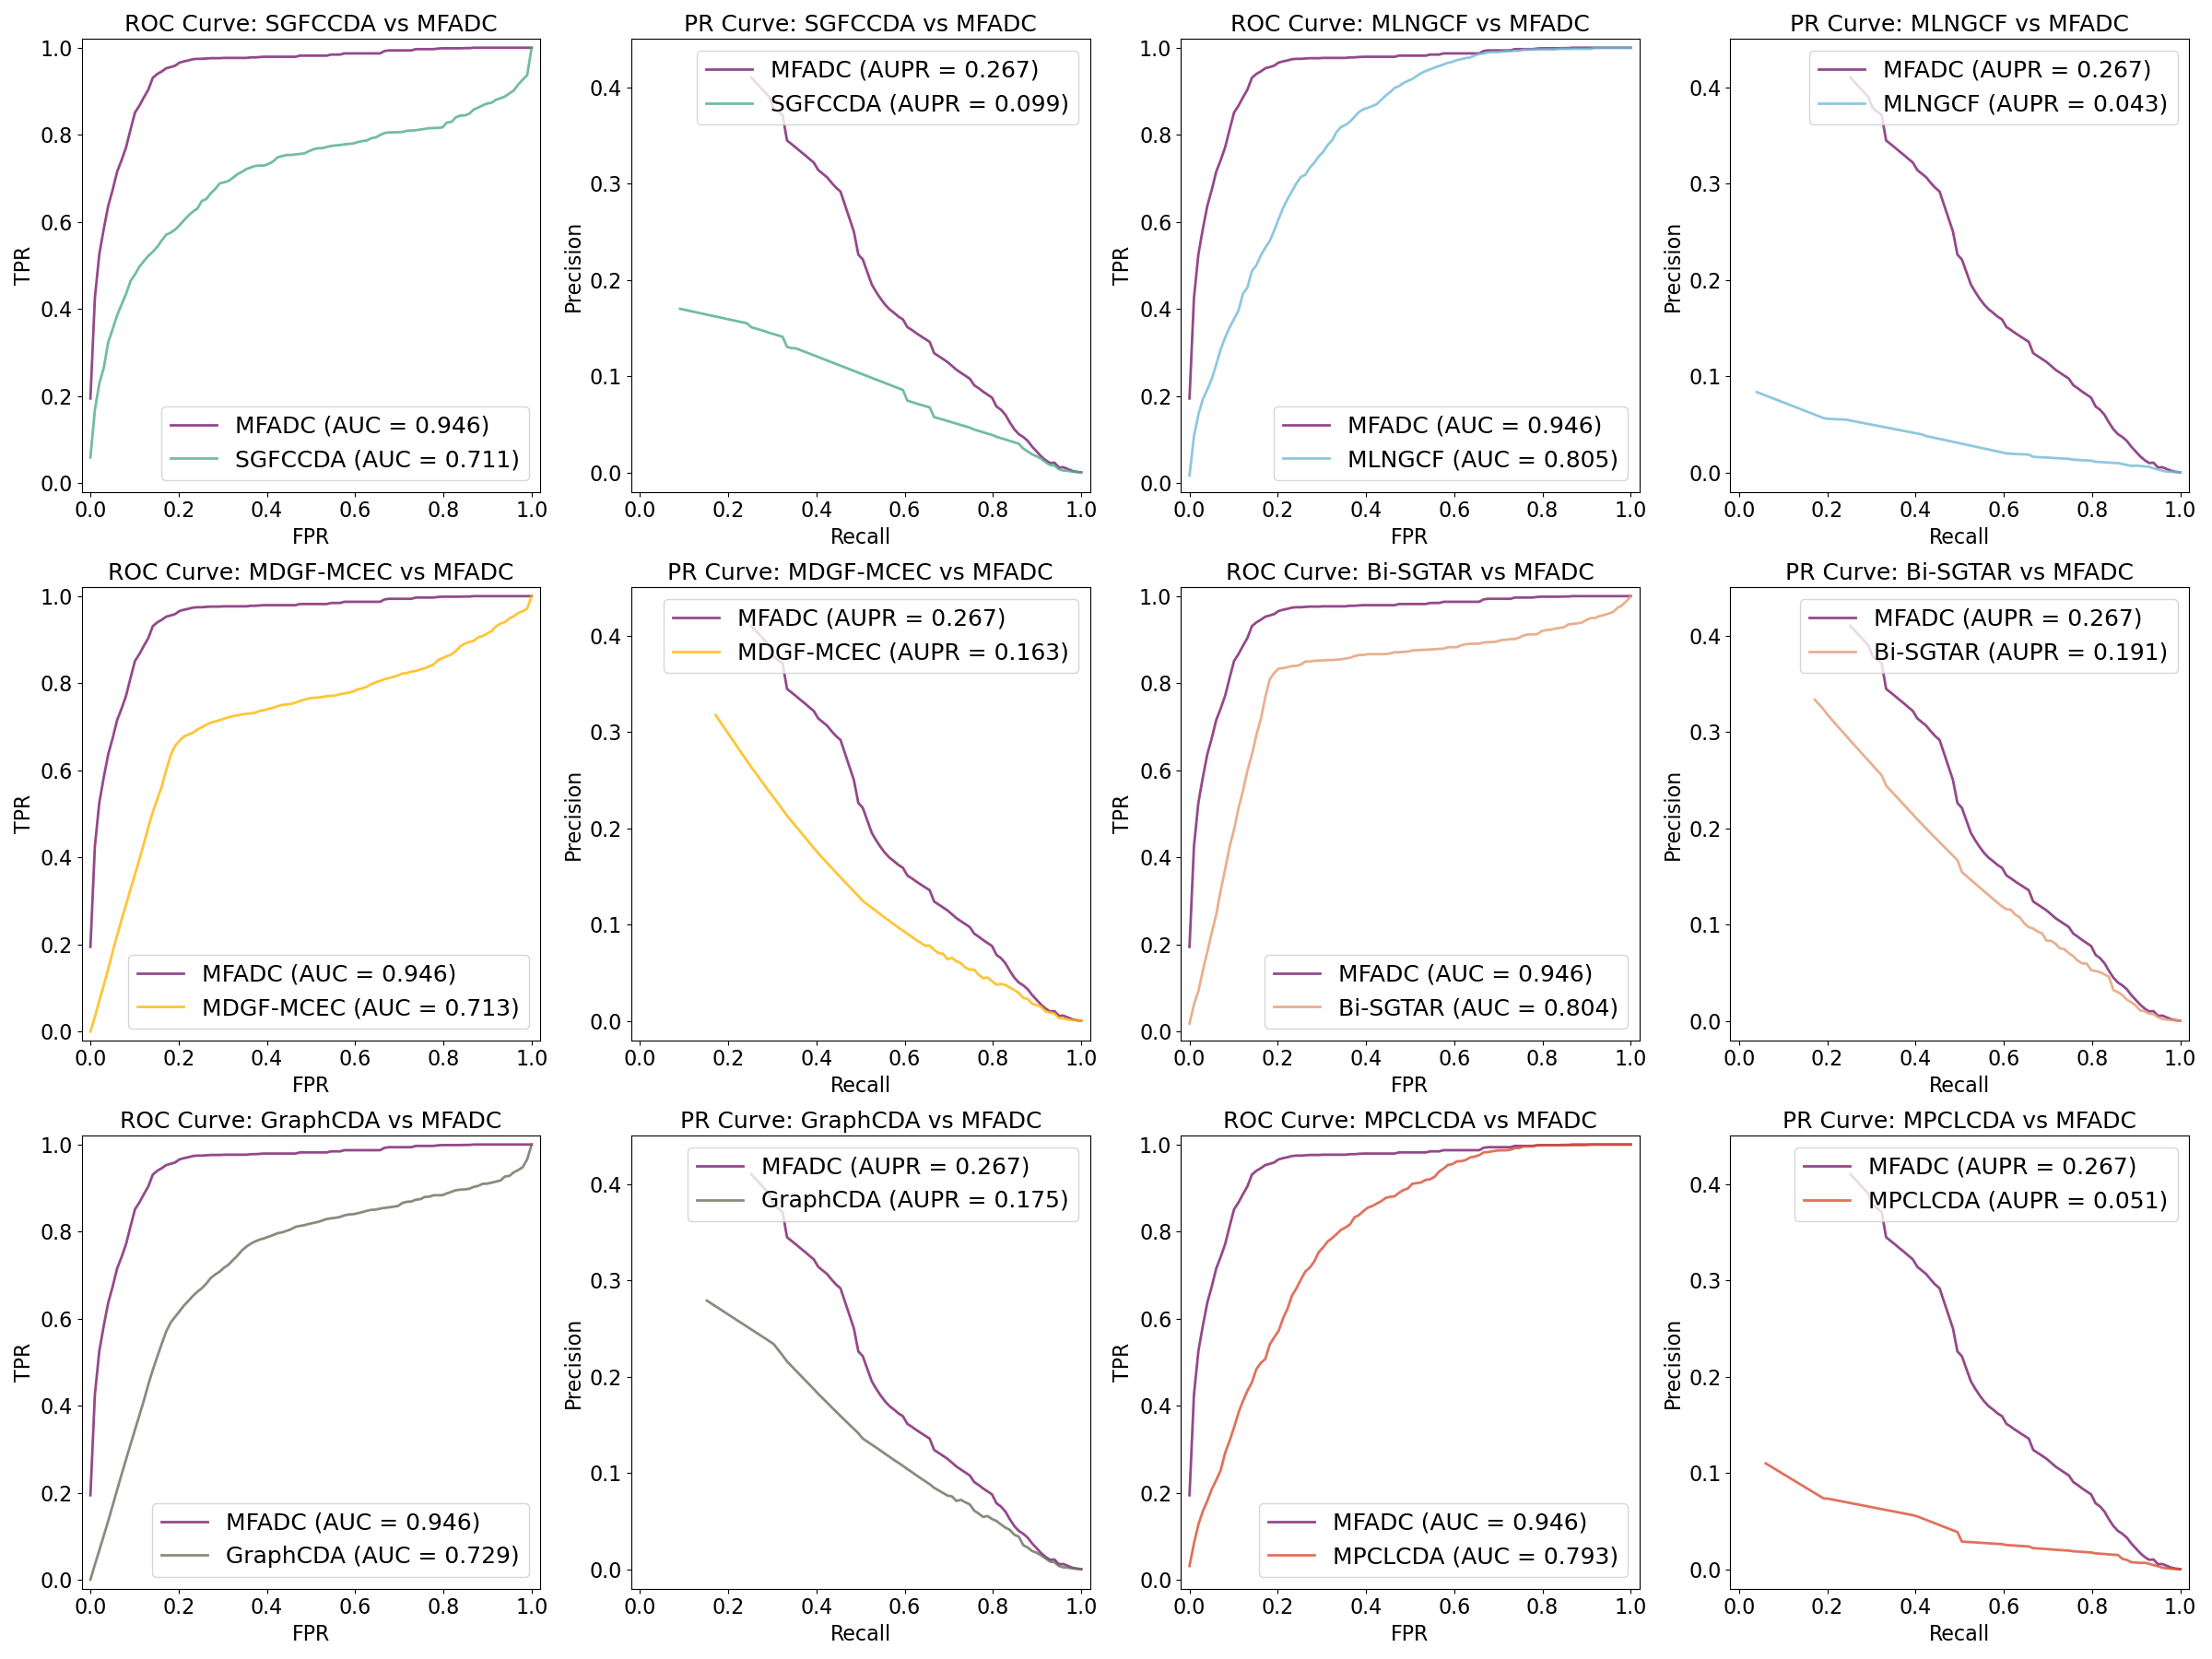
\includegraphics[width=8in]{fig/roc_pr_split.png}
    \caption{ROC and PR curves of MKCD and other methods.}
    \label{fig:roc_pr_split}
\end{figure*}

\begin{table*}[!t]
	\label{tab:02}
	\centering
	\begin{threeparttable}[b]
		\vspace{0.4cm}
		\renewcommand{\arraystretch}{1.3}  % 增大行高
		\caption{Results of the paired Wilcoxon test by comparing MKCD and any of the other methods.  }\label{tab:tab2}
        \setlength{\tabcolsep}{0pt}  % 调整列间距,适当增加空白
		\begin{tabular}{p{3.0cm}<{\centering}  p{2.9cm}<{\centering} p{2.9cm}<{\centering} p{2.9cm}<{\centering} p{2.9cm}<{\centering} p{2.9cm}<{\centering} p{2.9cm}<{\centering}}
			\hline
            \textbf{$p\ $-value} & \textbf{SGFCCDA} & \textbf{MLNGCF} & \textbf{MDGF-MCEC} &  \textbf{Bi-SGTAR} & \textbf{GraphCDA} & \textbf{MPCLCDA}\\
			\hline
		    AUC & 2.71e-111 & 7.20e-58 & 2.13e-109 &  3.27e-60 & 6.06e-108 & 1.22e-76 \\
		    AUPR & 6.02e-109 & 6.60e-115 & 1.18e-41 &  1.96e-09 & 2.86e-26 & 1.29e-113 \\
			\hline
		\end{tabular}
	\end{threeparttable}
	\vspace{-0.1cm}
\end{table*}

We compared MKCD with six advanced methods for predicting circRNA-disease associations, including SGFCCD \cite{shang2024sgfccda}, MLNGCF \cite{wu2023mlngcf}, MDGF-MCEC \cite{wu2022mdgf}, Bi-SGTAR \cite{li2024bi}, GraphCDA \cite{dai2022graphcda}, and MPCLCDA \cite{liu2023mpclcda}. Each method was trained using the optimal parameters provided in their original papers, and the same training and testing datasets were utilized in cross-validation to ensure fairness.

SGFCCDA: This model constructs a circRNA-disease heterogeneous graph and predicts potential circRNA-disease associations through scale graph convolutional networks and convolutional neural networks.

MLNGCF: In this model, various similarities between circRNAs and diseases are utilized to estimate the association scores based on a multilayer attention neural network.

MDGF-MCEC: This method establishes relationship graphs for circRNAs and diseases based on their respective similarities and learns node features through a multi-view dual attention graph convolution network.

Bi-SGTAR: The adjacency matrix of the circRNA-disease heterogeneous graph is decomposed into two views, and an encoder with sparse gating is employed to identify all circRNA-disease associations.

GraphCDA: This approach constructs separate similarity networks for circRNAs and diseases, utilizing a hybrid graph embedding model that combines graph convolutional networks and graph attention networks to simultaneously learn feature representations for circRNAs and diseases.

MPCLCDA: It automatically selects meta-paths for constructing meta-path graphs and employs graph convolutional networks and contrastive learning to learn node features for circRNAs and diseases.

Figure \ref{fig:roc_pr_split} illustrates the ROC and PR curves for MKCD and the other methods. From the figure, it is evident that MKCD achieved the highest average AUC of 0.947, surpassing SGFCCDA by 23.5\%, MLNGCF by 14.1\%, MDGF-MCEC by 23.3\%, Bi-SGTAR by 14.2\%, GraphCDA by 21.7\%, and MPCLCDA by 15.3\%. The average AUPR of MKCD was 0.271, which is higher than SGFCCDA, MLNGCF, MDGF-MCEC, Bi-SGTAR, GraphCDA, and MPCLCDA by 17.2\%, 22.8\%, 10.8\%, 8.0\%, 9.6\%, and 22.0\%, respectively. Both MLNGCF and MPCLCDA employ graph neural networks, focusing solely on integrating the topology and node features of the circRNA-disease heterogeneous graph. In contrast to these two methods, SGFCCDA utilizes scale graph convolutional networks to address the issue of feature mixing between different channels caused by the linear layer structure of graph convolutional networks. MDGF-MCEC and GraphCDA primarily focus on learning from multiple similarity views, while Bi-SGTAR emphasizes learning from multiple heterogeneous graph views, which contributes to their higher AUPR. Our method outperforms these six methods mainly due to the embedding of multi-scale neighbor topology and the encoding of relationships among multiple features of circRNA, disease, and miRNA nodes.

\textcolor{blue}{For the prediction results of all 138 diseases, we employed the Paired Wilcoxon test to evaluate whether the performance of our method is significantly superior to those of the other six methods. According to the results in Table \ref{tab:tab2}, all $p$-values are less than 0.05, indicating that MKCD significantly outperforms SGFCCDA, MLNGCF, MDGF-MCEC, Bi-SGTAR, GraphCDA, and MPCLCDA in terms of AUC and AUPR.}

\textcolor{blue}{For each disease, we calculated the average recall rates of circRNA candidates at various top $k$ values (Figure \ref{fig:topK}). When $k = 30$, MKCD achieved a recall rate of 29.3\%, surpassing SGFCCDA by 12.1\%, MLNGCF by 15.2\%, MDGF-MCEC by 8.1\%, Bi-SGTAR by 8.0\%, GraphCDA by 9.1\%, and MPCLCDA by 15.1\%. When $k = 50$, 70, and 90, MKCD maintained its leading position with recall rates of 48.5\%, 68.6\%, and 90.1\%, respectively. Bi-SGTAR (41.3\%, 65.7\%, 89.8\%), MDGF-MCEC (41.3\%, 63.6\%, 87.9\%), and GraphCDA (39.4\%, 62.5\%, 88.8\%) also achieved decent performance. In contrast, SGFCCDA (29.3\%, 45.5\%, 70.6\%), MLNGCF (25.2\%, 39.4\%, 64.6\%), and MPCLCDA (25.3\%, 40.5\%, 66.7\%) shown inferior performance.}

\subsection{Case studies over three diseases}

\begin{figure*}[!t]
    \centering
    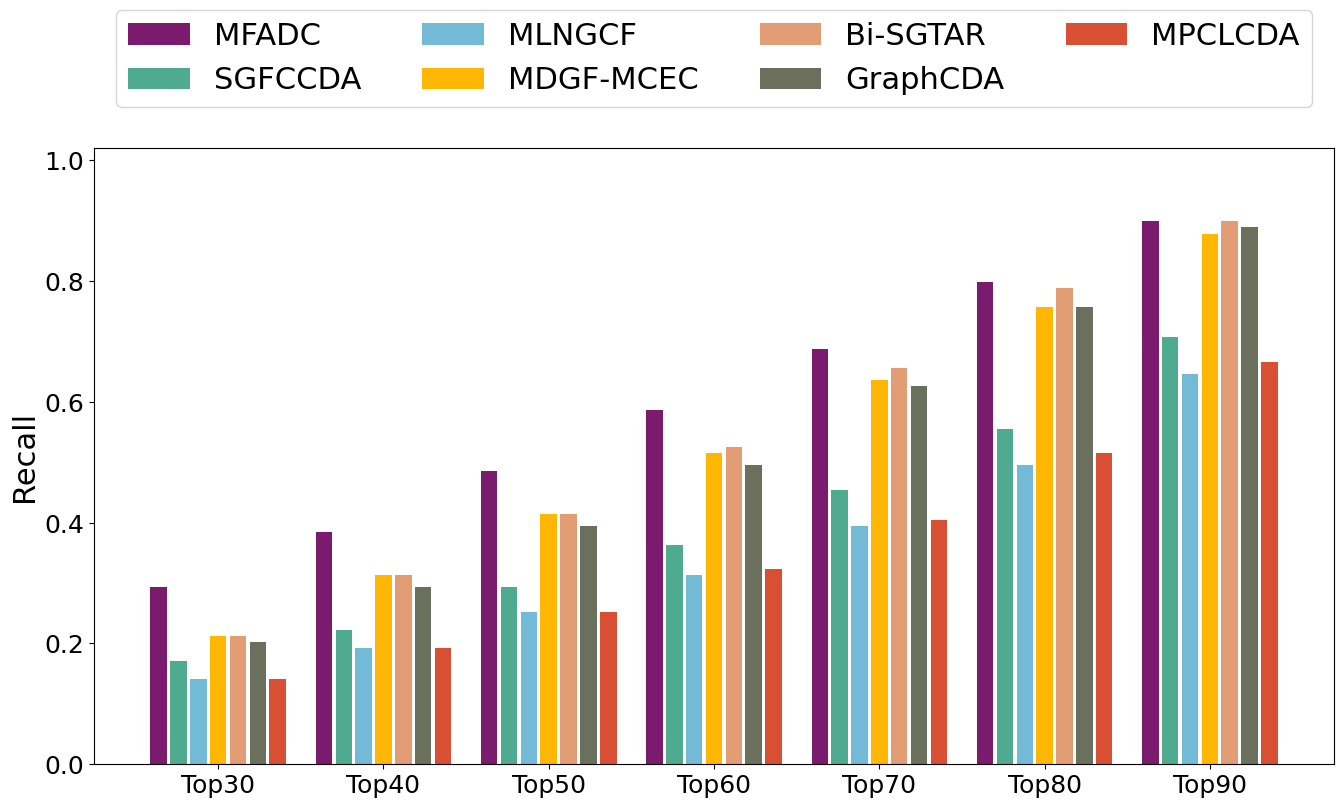
\includegraphics[width=6.5in]{fig/TopK_Recall.png}
     \caption{The average recall rates of diseases at multiple top k cutoffs}
    \label{fig:topK}
\end{figure*}

\textcolor{blue}{We conducted case studies on glioma, systemic lupus erythematosus, and glioblastoma to further validate the capability of MKCD in mining potential circRNA candidates associated with diseases. Glioma and glioblastoma are two types of primary brain tumors \cite{weller2015glioma, wirsching2017glioblastoma}, while systemic lupus erythematosus is a systemic autoimmune disease primarily affecting women \cite{borchers2010geoepidemiology}. For each disease, the circRNA candidates were ranked in descending order based on their association scores, and the top 15 circRNAs were selected as candidates. Tables \ref{tab:tab3}, \ref{tab:tab4}, and \ref{tab:tab5} present the top 15 circRNA candidates for glioma, systemic lupus erythematosus, and glioblastoma, respectively. \textcolor{blue}{The circRNADisease v2.0 database provides experimentally validated associations between circRNAs and various diseases, covering 4246 circRNAs and 330 diseases \cite{sun2024mode}. This database, along with relevant bioinformatics literature, was utilized to validate the predictions of circRNA-disease associations.}}

\begin{table*}[!t]
	\label{tab:03}
    \centering
    \begin{threeparttable}[b]  
        \caption{The top 15 predicted results of glioma-related circRNAs based on MKCD.}	\label{tab:tab3}
        \vspace{0.4cm}
        \setlength{\tabcolsep}{0pt}  % 调整列间距,适当增加空白
        \begin{tabular}{p{2cm}<{\centering} p{3.9cm}<{\raggedright} p{4.5cm}<{\raggedright} | p{2cm}<{\centering} p{3.9cm}<{\raggedright} p{4.2cm}<{\raggedright}}
            \hline
            \textbf{Rank} &  \textbf{circRNA name} & \textbf{Evidence} & \textbf{Rank} &  \textbf{circRNA name} & \textbf{Evidence} \\
            \hline
            1 & circ\_002136 & $L^a$, PMID:30736838 & 9 & hsa\_circ\_0079593 & $L^a$, PMID:31148222 \\
            2 & hsa\_circ\_0061868 & PMID:30341906 & 10 & circSMO742 & $L^a$, PMID:31895689 \\
            3 & circPTN & $L^a$, PMID:31511040 & 11 & hsa\_circ\_0012129 & $L^a$, PMID:29686222 \\
            4 & circ-TTBK2 & $L^a$, PMID:32196629 & 12 & hsa\_circ\_0088732 & $L^a$, PMID:32154171 \\
            5 & circ-EZH2 & $L^a$, PMID:31669648 & 13 & circNFIX & $L^a$, PMID:30072869 \\
            6 & hsa\_circ\_0000594 &  $L^a$, PMID:28219405 & 14 & circ-PTPRZ1 & $L^a$, PMID:31364003 \\
            7 & hsa\_circ\_0005198 & $L^a$, PMID:31038801 & 15 & hsa\_circ\_0014359 & $L^a$, PMID:30745107 \\
            8 & hsa\_circ\_0000177 & $L^a$, PMID:30010402 & & & \\
            \hline
        \end{tabular}
        \begin{tablenotes}
            \item $L^a$: circRNADisease v2.0.
        \end{tablenotes}
    \end{threeparttable}
    \vspace{-0.4cm}
\end{table*}

\begin{table*}[!t]
	\label{tab:04}
    \centering
    \begin{threeparttable}[b]  
        \caption{The top 15 predicted results of systemic lupus erythematosus-related circRNAs based on MKCD.}	\label{tab:tab4}
        \vspace{0.4cm}
        \setlength{\tabcolsep}{0pt}  % 调整列间距,适当增加空白
        \begin{tabular}{p{2cm}<{\centering} p{3.9cm}<{\raggedright} p{4.5cm}<{\raggedright} | p{2cm}<{\centering} p{3.9cm}<{\raggedright} p{4.2cm}<{\raggedright}}
            \hline
            \textbf{Rank} &  \textbf{circRNA name} & \textbf{Evidence} & \textbf{Rank} &  \textbf{circRNA name} & \textbf{Evidence} \\
            \hline
            1 & hsa\_circ\_0046599 & $L^a$, PMID:29360436 & 9 & hsa\_circ\_0008615 & $L^a$, PMID:29360436 \\
            2 & hsa\_circ\_0001866 & $L^a$, PMID:29360436 & 10 & hsa\_circ\_0021549 & $L^a$, PMID:29360436 \\
            3 & hsa\_circ\_0034398 & $L^a$, PMID:29360436 & 11 & has\_circ\_0049220 & $L^a$, PMID:29606700 \\
            4 & hsa\_circ\_0003146 & $L^a$, PMID:29360436 & 12 & hsa\_circ\_0092374 & $L^a$, PMID:29360436 \\
            5 & hsa\_circ\_0000479 & $L^a$, PMID:31608065 & 13 & hsa\_circ\_0040705 & $L^a$, PMID:29360436 \\
            6 & hsa\_circ\_0057762 & $L^a$, PMID:30628013 & 14 & hsa\_circ\_0012919 & $L^a$, PMID:30237316 \\
            7 & circPTPN22 & $L^a$, PMID:30871426 & 15 & hsa\_circ\_0049224 & $L^a$, PMID:29606700 \\
            8 & hsa\_circ\_0045272 & $L^a$, PMID:29700819 & & & \\
            \hline
        \end{tabular}
        \begin{tablenotes}
            \item $L^a$: circRNADisease v2.0.
        \end{tablenotes}
    \end{threeparttable}
    \vspace{-0.4cm}
\end{table*}

\begin{table*}[!t]
	\label{tab:05}
    \centering
    \begin{threeparttable}[b]  
        \caption{The top 15 predicted results of glioblastoma-related circRNAs based on MKCD.}	\label{tab:tab5}
        \vspace{0.4cm}
        \setlength{\tabcolsep}{0pt}  % 调整列间距,适当增加空白
        \begin{tabular}{p{2cm}<{\centering} p{3.9cm}<{\raggedright} p{4.5cm}<{\raggedright} | p{2cm}<{\centering} p{3.9cm}<{\raggedright} p{4.2cm}<{\raggedright}}
            \hline
            \textbf{Rank} &  \textbf{circRNA name} & \textbf{Evidence} & \textbf{Rank} &  \textbf{circRNA name} & \textbf{Evidence} \\
            \hline
            1 & hsa\_circ\_0001801 & $L^a$, PMID:31858556 & 9 & circMTO1 & $L^a$, PMID:31456594 \\
            2 & circNT5E & $L^a$, PMID:29967262 & 10 & circ-AKT3 & $L^a$, PMID:31470874 \\
            3 & circ-PITX1 & $L^a$, PMID:31493405 & 11 & circPVT1 & unknown \\
            4 & hsa\_circ\_0043949 & $L^a$, PMID:31823158 & 12 & circPTN & $L^a$, PMID:31511040 \\
            5 & hsa\_circ\_0074027 & $L^a$, PMID:30738578 & 13 & hsa\_circ\_101996 & unknown \\
            6 & circMMP9 & $L^a$, PMID:30470262 & 14 & hsa\_circ\_100242 & unknown \\
            7 & circ-Foxo3 & $L^a$, PMID:31802888 & 15 & hsa\_circ\_0003855 & unknown \\
            8 & hsa\_circ\_0001946 & $L^a$, PMID:31599076 & & & \\
            \hline
        \end{tabular}
        \begin{tablenotes}
            \item $L^a$: circRNADisease v2.0.
        \end{tablenotes}
    \end{threeparttable}
    \vspace{-0.4cm}
\end{table*}

\textcolor{blue}{Taking glioma as an example (Table \ref{tab:tab3}), all 15 circRNAs have been validated in the literature, \textcolor{blue}{with 14 of them being identified in circRNADisease v2.0}. For instance, the top-ranked hsa\_circ\_002136 was discovered by He et al. \cite{he2019fus} to inhibit the survival, migration, and tube formation of U87 glioma-exposed endothelial cells (GECs). The second-ranked hsa\_circ\_0061868 was found by Li et al. \cite{li2019circ} to be upregulated in glioma (the expression levels of hsa\_circ\_0061868 ... were upregulated).}

\textcolor{blue}{The top 15 circRNA candidates associated with systemic lupus erythematosus (SLE) (Table \ref{tab:tab4}) have all been confirmed in the literature, \textcolor{blue}{and are included in circRNADisease v2.0}. For example, Li et al. \cite{li2018comprehensive} identified hsa\_circ\_0046599 as a potential biomarker for systemic lupus erythematosus. hsa\_circ\_0000479 was confirmed by Guo et al. \cite{guo2019hsa_circ_0000479} to be upregulated in peripheral blood mononuclear cells of patients with SLE.}

\textcolor{blue}{\textcolor{blue}{For glioblastoma, 11 of the top 15 circRNA candidates (Table \ref{tab:tab5}) have been validated in recent literature as well as in circRNADisease v2.0}. For example, the study by Wang et al. \cite{wang2018circnt5e} demonstrated that circNT5E exhibits tumor suppressor-like features in glioblastoma. Additionally, circMMP9 was shown by Wang et al. \cite{wang2018eif4a3} to promote the proliferation, migration, and invasion capabilities of glioblastoma multiforme cells.}


\subsection{Prediction of novel circRNA-disease associations}
\textcolor{blue}{We utilized all known associations between circRNAs and diseases, and randomly selected an equal number of negative examples to train MKCD for predicting circRNA candidates for 138 diseases. The top 15 circRNA candidates predicted by MKCD for each disease are listed in \href{path/to/S1.pdf}{Supplementary File S1}.}


%---------------------------------------------------------------------------------------------------------------------


\section{Conclusion}
This paper introduces a novel approach for encoding the relationships among circRNA, miRNA, and disease node features, as well as learning and integrating the global and local features of node pairs to predict disease-related circRNAs. By adjusting the walking range of random walkers in the circRNA-disease-miRNA heterogeneous graph, we construct multi-scale neighbor topologies, with the importance of each scale neighbor topology being adaptively determined. The designed multi-scale neighbor topology-guided transformer can dynamically update the neighbor topology and learn the dynamic relationships between the features of multiple circRNA, miRNA, and disease nodes. A feature-level gated network is established to assign higher weights to important topological and original features. The proposed ACK encodes the features of circRNA-disease node pairs, which helps to reveal the local and global dependencies between pairwise attributes. The results of five-fold cross-validation experiments demonstrated that the AUC and AUPR of MKCD are higher than those of six comparative methods. The recall rate of top-ranked circRNA candidates and case studies over three diseases indicate that MKCD is capable of providing reliable disease-related circRNA candidates.


\end{methods}

% \setlength{\fboxrule}{1pt}
\begin{thebibliography}{}
\normalsize
%1
\bibitem{jeck2014detecting}
Jeck W R, Sharpless N E. Detecting and characterizing circular RNAs. Nature biotechnology, 2014, 32(5): 453-461.
%2%4
\bibitem{abdelmohsen2017identification}
Abdelmohsen K, Panda A C, Munk R, et al. Identification of HuR target circular RNAs uncovers suppression of PABPN1 translation by CircPABPN1. RNA biology, 2017, 14(3): 361-369.
%5
\bibitem{gao2019circular}
Gao S, Yu Y, Liu L, et al. Circular RNA hsa\_circ\_0007059 restrains proliferation and epithelial-mesenchymal transition in lung cancer cells via inhibiting microRNA-378. Life sciences, 2019, 233: 116692.
%6
\bibitem{li2019tumor}
Li Z, Ruan Y, Zhang H, et al. Tumor‐suppressive circular RNAs: mechanisms underlying their suppression of tumor occurrence and use as therapeutic targets. Cancer science, 2019, 110(12): 3630-3638.
%7
\bibitem{liang2020autophagy}
Liang G, Ling Y, Mehrpour M, et al. Autophagy-associated circRNA circCDYL augments autophagy and promotes breast cancer progression. Molecular cancer, 2020, 19: 1-16.
%8
\bibitem{wang2018circibtk}
Wang X, Zhang C, Wu Z, et al. CircIBTK inhibits DNA demethylation and activation of AKT signaling pathway via miR-29b in peripheral blood mononuclear cells in systemic lupus erythematosus. Arthritis Research \& Therapy, 2018, 20: 1-10.
%9
\bibitem{khan2016rbm20}
Khan M A F, Reckman Y J, Aufiero S, et al. RBM20 regulates circular RNA production from the titin gene. Circulation research, 2016, 119(9): 996-1003.
%10
\bibitem{siede2017identification}
Siede D, Rapti K, Gorska A A, et al. Identification of circular RNAs with host gene-independent expression in human model systems for cardiac differentiation and disease. Journal of molecular and cellular cardiology, 2017, 109: 48-56.
%11
\bibitem{jin2019silencing}
Jin C, Zhao W, Zhang Z, et al. Silencing circular RNA circZNF609 restrains growth, migration and invasion by up-regulating microRNA-186-5p in prostate cancer. Artificial cells, nanomedicine, and biotechnology, 2019, 47(1): 3350-3358.
%12
\bibitem{lan2023benchmarking}
Lan W, Dong Y, Zhang H, et al. Benchmarking of computational methods for predicting circRNA-disease associations. Briefings in Bioinformatics, 2023, 24(1): bbac613.
%
\bibitem{yang2021predicting}
Yang J, Lei X. Predicting circRNA-disease associations based on autoencoder and graph embedding. Information Sciences, 2021, 571: 323-336.
%13
\bibitem{fan2018prediction}
Fan C, Lei X, Wu F X. Prediction of CircRNA-disease associations using KATZ model based on heterogeneous networks. International journal of biological sciences, 2018, 14(14): 1950.
%14
\bibitem{lei2018pwcda}
Lei X, Fang Z, Chen L, et al. PWCDA: path weighted method for predicting circRNA-disease associations. International journal of molecular sciences, 2018, 19(11): 3410.
%14
\bibitem{wei2020icircda}
Wei H, Liu B. iCircDA-MF: identification of circRNA-disease associations based on matrix factorization. Briefings in bioinformatics, 2020, 21(4): 1356-1367.
%15
\bibitem{wang2022combining}
Wang M N, Xie X J, You Z H, et al. Combining K nearest neighbor with nonnegative matrix factorization for predicting circrna-disease associations. IEEE/ACM Transactions on Computational Biology and Bioinformatics, 2022, 20(5): 2610-2618.
%
\bibitem{lei2020integrating}
Lei X, Bian C. Integrating random walk with restart and k-Nearest Neighbor to identify novel circRNA-disease association. Scientific reports, 2020, 10(1): 1943.
%16
\bibitem{yan2018dwnn}
Yan C, Wang J, Wu F X. DWNN-RLS: regularized least squares method for predicting circRNA-disease associations. BMC bioinformatics, 2018, 19: 73-81.
%16
\bibitem{wang2022machine}
Wang L, Wong L, Li Z, et al. A machine learning framework based on multi-source feature fusion for circRNA-disease association prediction. Briefings in Bioinformatics, 2022, 23(5): bbac388.
%17
\bibitem{lei2019gbdtcda}
Lei X, Fang Z. GBDTCDA: predicting circRNA-disease associations based on gradient boosting decision tree with multiple biological data fusion. International journal of biological sciences, 2019, 15(13): 2911.
%
\bibitem{deepthi2021inferring}
Deepthi K, Jereesh A S. Inferring potential CircRNA–disease associations via deep autoencoder-based classification. Molecular Diagnosis \& Therapy, 2021, 25: 87-97.
%18
\bibitem{peng2022rnmflp}
Peng L, Yang C, Huang L, et al. RNMFLP: predicting circRNA–disease associations based on robust nonnegative matrix factorization and label propagation. Briefings in bioinformatics, 2022, 23(5): bbac155.
%
\bibitem{zhang2019predicting}
Zhang W, Yu C, Wang X, et al. Predicting CircRNA-disease associations through linear neighborhood label propagation method. Ieee Access, 2019, 7: 83474-83483.
%
\bibitem{tian2024mamlcda}
Tian Y, Zou Q, Wang C Y, et al. MAMLCDA: A Meta-Learning Model for Predicting circRNA-Disease Association Based on MAML Combined With CNN. IEEE Journal of Biomedical and Health Informatics, 2024.
%
\bibitem{wang2020efficient}
Wang L, You Z H, Huang Y A, et al. An efficient approach based on multi-sources information to predict circRNA–disease associations using deep convolutional neural network. Bioinformatics, 2020, 36(13): 4038-4046.
%
\bibitem{lu2020improving}
Lu C, Zeng M, Wu F X, et al. Improving circRNA–disease association prediction by sequence and ontology representations with convolutional and recurrent neural networks. Bioinformatics, 2020, 36(24): 5656-5664.
%
\bibitem{li2024bi}
Li S, Chen Q, Liu Z, et al. Bi-SGTAR: A simple yet efficient model for circRNA-disease association prediction based on known association pair only. Knowledge-Based Systems, 2024, 291: 111622.
%21
\bibitem{shang2024sgfccda}
Shang J, Zhao L, He X, et al. SGFCCDA: Scale Graph Convolutional Networks and Feature Convolution for circRNA-Disease Association Prediction. IEEE Journal of Biomedical and Health Informatics, 2024.
%24
\bibitem{liu2023mpclcda}
Liu W, Tang T, Lu X, et al. MPCLCDA: predicting circRNA–disease associations by using automatically selected meta-path and contrastive learning. Briefings in Bioinformatics, 2023, 24(4): bbad227.
%23
\bibitem{wu2022mdgf}
Wu Q, Deng Z, Pan X, et al. MDGF-MCEC: a multi-view dual attention embedding model with cooperative ensemble learning for CircRNA-disease association prediction. Briefings in Bioinformatics, 2022, 23(5): bbac289.
%19
\bibitem{wu2023mlngcf}
Wu Q, Deng Z, Zhang W, et al. MLNGCF: circRNA–disease associations prediction with multilayer attention neural graph-based collaborative filtering. Bioinformatics, 2023, 39(8): btad499.
%22
\bibitem{dai2022graphcda}
Dai Q, Liu Z, Wang Z, et al. GraphCDA: a hybrid graph representation learning framework based on GCN and GAT for predicting disease-associated circRNAs. Briefings in Bioinformatics, 2022, 23(5): bbac379.
%32
\bibitem{liu2024kan}
Liu Z, Wang Y, Vaidya S, et al. Kan: Kolmogorov-arnold networks. arXiv preprint arXiv:2404.19756, 2024.
%
\bibitem{lan2022kgancda}
Lan W, Dong Y, Chen Q, {\it et al.} KGANcDA: a knowledge graph attention network for lncRNA-disease association prediction. {\it Briefings in Bioinformatics} 2022;23(1):bbab494.
%26
\bibitem{lan2020circr2cancer}
Lan W, Zhu M, Chen Q, {\it et al.} CircR2Cancer: a manually curated database of associations between circRNAs and cancers. {\it Database} 2020;2020:baaa085.
%27
\bibitem{rophina2020circad}
Rophina M, Sharma D, Poojary M, {\it et al.} CircAD: a comprehensive database for differentially expressed circRNAs associated with various diseases. {\it Database} 2020;2020:baaa019.
%28
\bibitem{zhao2018circrna}
Zhao Z, Wang K, Wu F, {\it et al.} circRNA disease: a manually curated database of experimentally supported circRNA-disease associations. {\it Cell Death \& Disease} 2018;9(5):475.
%29
\bibitem{wang2010inferring}
Wang D, Wang J, Lu M, {\it et al.} Inferring the human microRNA functional similarity and functional network based on microRNA-associated diseases. {\it Bioinformatics} 2010;26(13):1644-1650.
%30
\bibitem{chen2015constructing}
Chen X, Clarence Yan C, Luo C, {\it et al.} Constructing lncRNA functional similarity network based on lncRNA-disease associations and disease semantic similarity. {\it Scientific reports} 2015;5:11338
%31
\bibitem{vaswani2017attention}
Vaswani A. Attention is all you need. Advances in Neural Information Processing Systems, 2017.

%33
\bibitem{hajian2013receiver}
Hajian-Tilaki K. Receiver operating characteristic (ROC) curve analysis for medical diagnostic test evaluation. Caspian journal of internal medicine, 2013, 4(2): 627.
%34
\bibitem{saito2015precision}
Saito T, Rehmsmeier M. The precision-recall plot is more informative than the ROC plot when evaluating binary classifiers on imbalanced datasets. PloS one, 2015, 10(3): e0118432.
%
\bibitem{weller2015glioma}
Weller M, Wick W, Aldape K, et al. Glioma. Nature reviews Disease primers, 2015, 1(1): 1-18.
%
\bibitem{wirsching2017glioblastoma}
Wirsching H G, Weller M. Glioblastoma. Malignant Brain Tumors: State-of-the-Art Treatment, 2017: 265-288.
%
\bibitem{borchers2010geoepidemiology}
Borchers A T, Naguwa S M, Shoenfeld Y, et al. The geoepidemiology of systemic lupus erythematosus. Autoimmunity reviews, 2010, 9(5): A277-A287.
%35
\bibitem{sun2024mode}
Sun Z Y, Yang C L, Huang L J, et al. circRNADisease v2.0: an updated resource for high-quality experimentally supported circRNA-disease associations. Nucleic Acids Research, 2024, 52(D1): D1193-D1200.
%
\bibitem{he2019fus}
He Z, Ruan X, Liu X, et al. FUS/circ\_002136/miR-138-5p/SOX13 feedback loop regulates angiogenesis in Glioma. Journal of Experimental \& Clinical Cancer Research, 2019, 38: 1-19.
%36
\bibitem{li2019circ}
Li G, Huang M, Cai Y, et al. Circ‐U2AF1 promotes human glioma via derepressing neuro‐oncological ventral antigen 2 by sponging hsa‐miR‐7‐5p. Journal of Cellular Physiology, 2019, 234(6): 9144-9155.
%37
\bibitem{li2018comprehensive}
Li H, Li K, Lai W, et al. Comprehensive circular RNA profiles in plasma reveals that circular RNAs can be used as novel biomarkers for systemic lupus erythematosus. Clinica Chimica Acta, 2018, 480: 17-25.
%38
\bibitem{guo2019hsa_circ_0000479}
Guo G, Wang H, Ye L, et al. Hsa\_circ\_0000479 as a novel diagnostic biomarker of systemic lupus erythematosus. Front Immunol 10: 2281.(2019)
%39
\bibitem{wang2018circnt5e}
Wang R, Zhang S, Chen X, et al. CircNT5E acts as a sponge of miR-422a to promote glioblastoma tumorigenesis. Cancer research, 2018, 78(17): 4812-4825.
%40
\bibitem{wang2018eif4a3}
Wang R, Zhang S, Chen X, et al. EIF4A3-induced circular RNA MMP9 (circMMP9) acts as a sponge of miR-124 and promotes glioblastoma multiforme cell tumorigenesis. Molecular cancer, 2018, 17: 1-12.
\end{thebibliography}

\end{document}
